%-----------------------------------------------------------%
% Propuesta de plantilla en LaTeX para tesis formato UAG    %
% Autor: Jose Francisco Rosales Fonseca                     % 
% Contacto: francofonseca501@gmail.com                      %
% Fecha: Diciembre  2022                                    %
%-----------------------------------------------------------%
% El objetivo de esta plantilla es facilitar la redacción   %
% en LaTeX de tu tesis siguiendo los lineamientos de la UAG.%
% Mi intención es pues que se dedique el tiempo al          %
% contenido de la tesis evitando las largas horas           %
% entendiendo LaTeX.                                        %  
% Siéntete libre de modificar la plantilla de acuerdo a tus %
% necesidades.                                              %
%-----------------------------------------------------------%
% Utiliza el libro libro LaTeX_2014.pdf que se encuentra    %
% dentro de la carpeta "ayuda" para más información.        %
%-----------------------------------------------------------%

%-----------------------------------------------------------%
% Las siguientes configuraciones son con el objetivo de una
% tesis en español siguiendo los lineamientos estipulados
% en: http://crecea.uag.mx/opciones/tesis.htm
% En relación al diseño de la portada los lineamientos 
% estipulados en: http://crecea.uag.mx/opciones/portada.htm

    \documentclass[12pt,twoside]{report}
    \usepackage[T1]{fontenc}
    \usepackage[utf8]{inputenc} % only needed for older LaTeX
    \usepackage{pdfpages}
    \usepackage{longtable,multirow,booktabs}
    \usepackage{setspace}
    \usepackage{graphicx}
    \usepackage{cite}
    \usepackage{tabu}
    \usepackage[spanish, es-tabla]{babel}
    \usepackage{amssymb}
    \usepackage{amsmath}
    \usepackage{esvect}
    \usepackage{hyperref}
    \usepackage[a4paper,width=150mm,top=25mm,bottom=25mm,bindingoffset=6mm]{geometry} %Formato márgenes, etc.
    \usepackage[font=footnotesize,labelfont=bf]{caption}
    \usepackage{minted}
    \usepackage{tikz}
    \usepackage{verbatim}
    \usepackage[nopostdot,acronym,toc,section=chapter,style=indexgroup,nomain]{glossaries}
    \usepackage{listings}
    \usepackage{xcolor}
    \usepackage{contraportada/glosario}
    \usepackage{contraportada/urls}
    \usepackage{float}
    \makeglossaries

    \graphicspath{{imagenes/}} %Ubicación de imágenes
    \hypersetup{
        %Configuración comandos de referencia cruzada en LATEX:
        colorlinks=true,
        linkcolor=black,
        citecolor=blue,
        filecolor=blue,
        urlcolor=blue,
        %Opciones de visualización e información PDF:
        pdfauthor={"Jose Francisco Rosales Fonseca"},
        pdftitle={"Configuración de un servidor Linux para el manejo de nodos a través del protocolo LoRaWAN."},
        pdfsubject={"Configuración de un servidor Linux para el manejo de nodos a través del protocolo LoRaWAN."},
        pdfcreator={"Jose Francisco Rosales Fonseca"},
        pdfproducer={"Jose Francisco Rosales Fonseca"},
        pdfkeywords={"Linux, LoRaWAN, IoT, The-Things-Stack, Linux, Docker"}
    }

    \begin{document}

        \lstset{basicstyle=\ttfamily,
showstringspaces=false, commentstyle=\color{red}, keywordstyle=\color{blue} }

        %Carátula de tesis

\begin{titlepage}
    \begin{center}
        \rule{\textwidth}{4pt}\vspace*{-\baselineskip}\vspace*{2pt} % Thick horizontal line
        \rule{\textwidth}{1pt}\\[\baselineskip] % Thin horizontal line
        \textbf{\normalsize UNIVERSIDAD AUTÓNOMA DE GUADALAJARA} % Title
        \rule{\textwidth}{0.4pt}\vspace*{-\baselineskip}\vspace{3.2pt} % Thin horizontal line
        \rule{\textwidth}{1.6pt}\\[\baselineskip] % Thick horizontal line
        
        {\tiny CON RECONOCIMIENTO DE VALIDEZ OFICIAL DE ESTUDIOS DE LA SECRETARÍA DE \\ EDUCACIÓN PÚBLICA SEGÚN ACUERDO No.158 DE FECHA 17 DE JULIO DE 1991} % Title
        \rule{\textwidth}{0.4pt}\vspace*{-\baselineskip}\vspace{3.2pt} % Thin horizontal line
        \rule{\textwidth}{1.6pt}\\[\baselineskip] % Thick horizontal line

        \textbf{\small POSGRADO E INVESTIGACIÓN} % Title
        
        \vspace*{1.2cm}
        
\includegraphics[width=0.3\textwidth]{uag_2.jpg}
        \vspace*{1.2cm}
        
        {\small Servidor LoRa para redes inalámbricas de sensores de largo alcance y baja potencia }
        \rule{\textwidth}{0.6pt}\\[\baselineskip] % Thick horizontal line
        
        \textbf{\small TESIS} % Title
        \vspace*{1.2cm} 
        
        {\scriptsize QUE PRESENTA}
        
        \textbf{\scriptsize JOSÉ FRANCISCO ROSALES FONSECA }
        \vspace*{1.2cm}
        
        {\scriptsize PARA OBTENER EL GRADO DE}
        
        \textbf{\small MAESTRÍA EN CIENCIAS COMPUTACIONALES} % Title
        \vspace*{1.2cm}
        
        {\scriptsize DIRECTOR DE TESIS:\\  DRA LINA MARIA AGUILAR LOBO}
        
        \vfill
        
        {\scriptsize GUADALAJARA, JALISCO. AGOSTO 2023 \\ Número de registro en el sistema de investigación}
        \rule{\textwidth}{4pt}\vspace*{-\baselineskip}\vspace*{2pt} % Thick horizontal line
    \end{center}
\end{titlepage}

        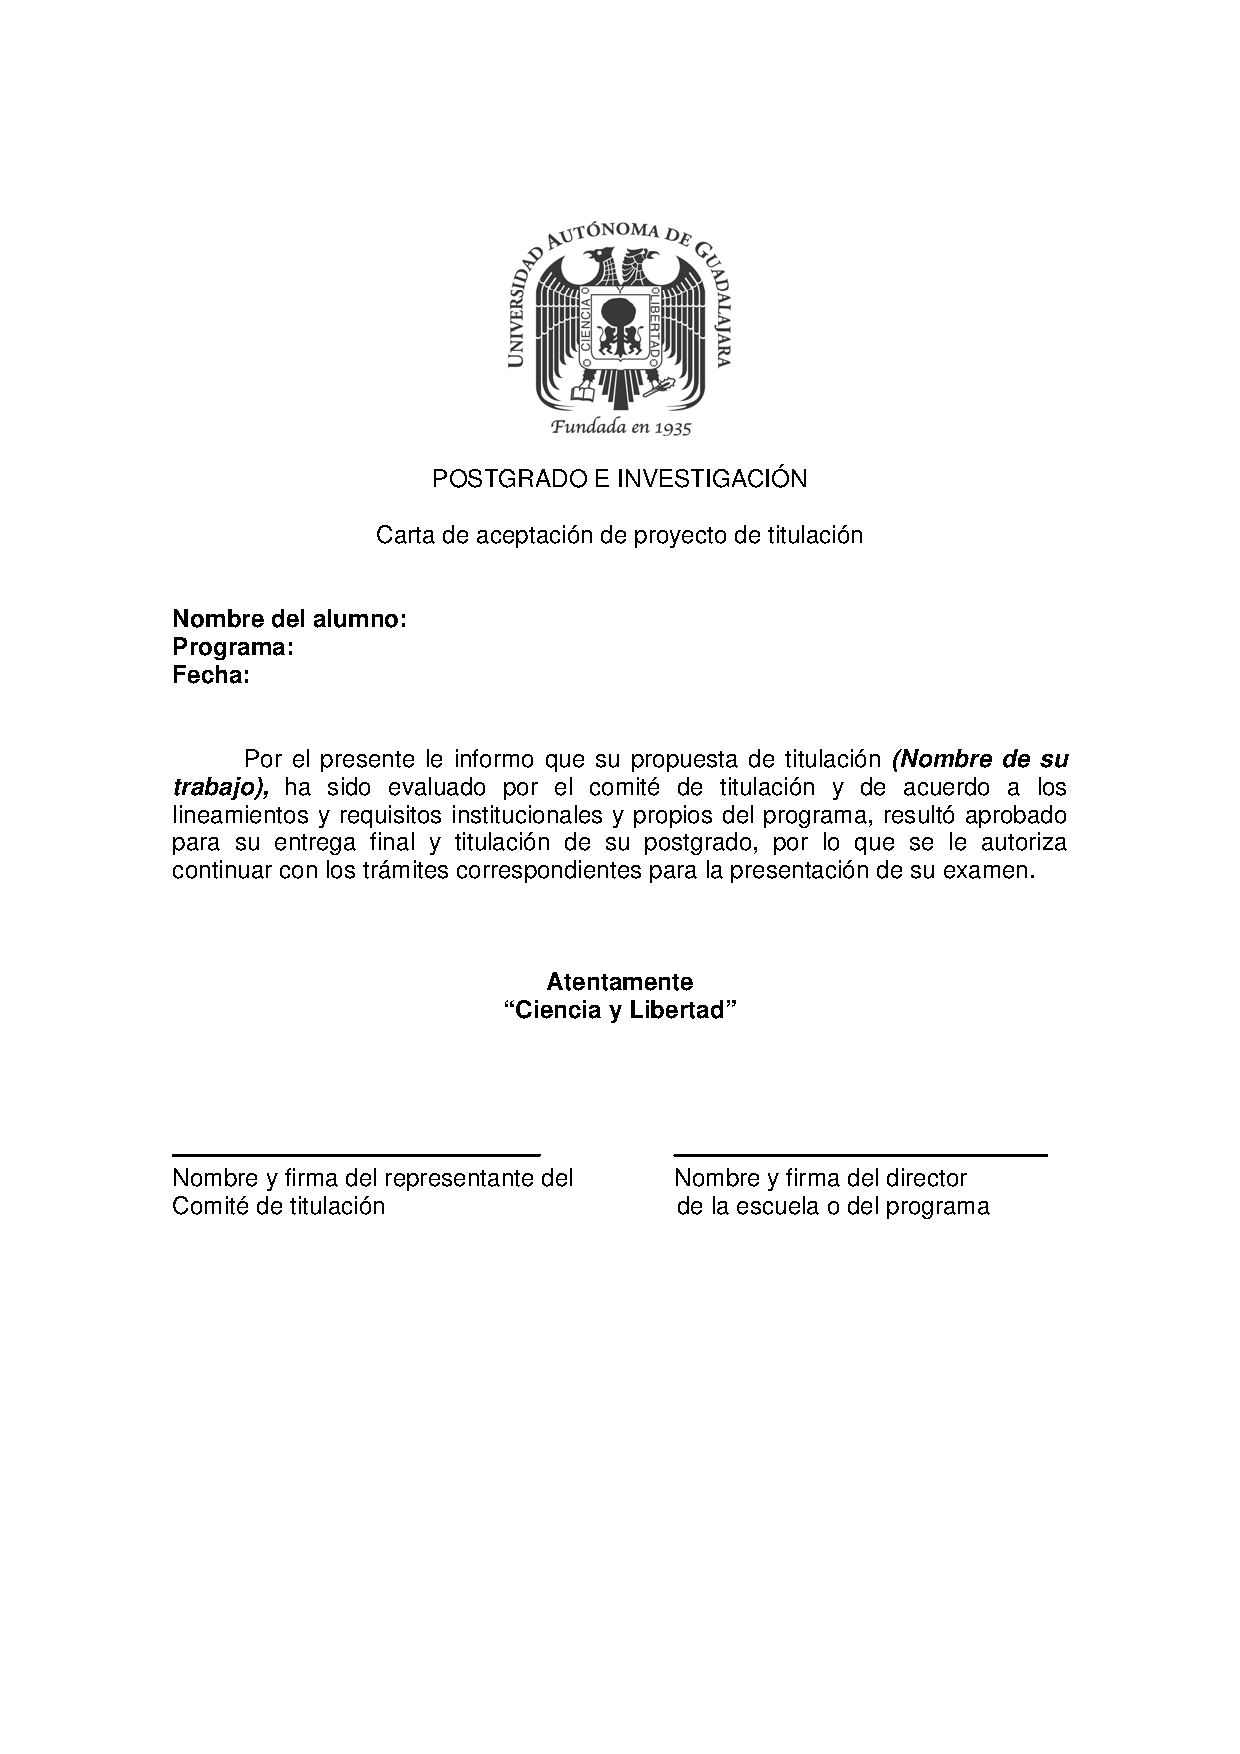
\includepdf[]{portada/cartaaceptacion.pdf} %archivo PDF y nombre de tu carta de aceptación

        \spacing{1.5}

        \chapter*{Dedicatoria}
        %Dedicatoria

Dedico este trabajo a mi madre Angelica, por ser el pilar más importante en mi vida y por
demostrarme siempre su cariño y apoyo incondicional sin importar nuestras diferencias de opiniones.
A mis hermanas Dana y Angelica, que siempre han estado a mi lado apoyándome. A mis amigos Jahir,
Alex, Yoshua y Shannen que siempre han creído en mi y me han impulsado a volverme una mejor persona
y a perseguir mis sueños.
\\
\\
\emph{Los sueños comienzan cuando se cree en ellos.}


        \chapter*{Declaración expresa}
        %Declaración expresa

La responsabilidad por los hechos, ideas y doctrinas expuestas en este proyecto corresponden
exclusivamente a los directamente involucrados en su desarrollo, y el patrimonio intelectual de la
misma a la Universidad Autónoma de Guadalajara.


        \chapter*{Agradecimientos}
        % Agradecimientos

Antes que nada, agradezco a mi madre Angelica por todo el apoyo que siempre me ha brindado en todo
el transcurso de mi vida militar, mi vida civil, durante mis estudios, mi carrera profesional y en
lo largo de mi vida, sin ella este trabajo nunca hubiera sido posible.

También agradezco a mi asesora de tesis la Dra. Lina María Aguilar Lobo por su paciencia y sugerirme trabajar
en este proyecto además de sus revisiones constantes.
Así como a la Dra. Zaira Ruth Zuviria López por apoyarme fuera de clase con revisiones también de mi tesis y
su apoyo profesional y académico durante mis estudios. 

También agradezco a mis amigos y hermanos Jahir, Alex, Yoshua, Dana y Shannen por todo el apoyo que
de alguna u otra forma siempre me han dado, en mis momentos más bajos asi como en los más altos
gracias por estar ahí. Llevo en el corazón sus palabras de aliento y animo hacia mí.

Finalmente, a mi pareja Jacobien por apoyarme en finalizar de escribir mi proyecto y siempre alentándome a continuar mejorando.
\\
\\
\emph{Cuando ya el dolor te agobie y no puedas más seguir, descansar acaso debes, pero nunca desistir.}


        \tableofcontents

        \listoffigures

        %\listoftables
        \printglossaries

        \chapter{Introducción}
        %Capítulo 1

\section{Descripción del problema} \label{descripcionproblema}

En una red inalámbrica de sensores de largo alcance y baja potencia, específicamente en aplicaciones de \gls{iot} para ciudades inteligentes se tiene la necesidad de comunicar múltiples microcontroladores para la creación de una red de dispositivos que midan variables físicas en tiempo real y envíen esta información recolectada a un centro de control ubicado remotamente. Debido a la necesidad de un punto central que recabe todos estos datos es necesario la implementación de un servidor maestro el cual debe ser escalable, sencillo de configurar y a prueba de fallos. En este contexto, es igual de importante, contar con una documentación detallada en caso de enfrentar errores comunes o la necesidad de cambiar configuraciones, para que el servidor pueda ser restablecido bajo cualquier circunstancia de falla.

Por lo tanto, se requiere una solución a la necesidad de generar y configurar un servidor físico que funcione a manera de acceso entre un enrutador RG191 (de tecnología LoRa) y un microcontrolador STM32 núcleo L073RZ, así como un manual detallado de como replicarlo en caso de requerirlo.

\section{Definición del problema} \label{definicionproblema}

   
Diversos proyectos de Internet de las cosas para aplicaciones de ciudades inteligentes para realizar pruebas de concepto en un ambiente controlado, no cuentas con un servidor maestro para el enrutamiento de la red de dispositivos IoT.

\section{Objetivos del proyecto} \label{objetivoinvestigacion}


 \subsection{Objetivo General}
Implementar un servidor Linux que funcione a manera de puente entre un enrutador RG191 de tecnología LoRa y una red de sensores basada en un microcontrolador STM32 núcleo L073RZ, y crear un manual detallado de configuración. \\
\\
 \textbf{Objetivos específicos:}
 \begin{itemize}
  \item Configurar un servidor con un sistema operativo Linux así como todas las herramientas necesarias para su uso como puente entre enrutadores y nodos IoT utilizando el protocolo LoRaWAN. 
  \item Configurar un enrutador para el manejo y gestión de múltiples nodos LoRa tales como el alta y baja de dispositivos.
  \item Generar un manual detallado que abarque todos los problemas encontrados y el procedimiento para resolverlos.
\end{itemize}

\section{Delimitación } \label{delimitacioninvestigacion}


El alcance de este proyecto pasa por la generación de documento que cuente con las instrucciones necesarias para replicar la generación de servidores puentes, así como más enrutadores en caso de que la red se quiera escalar en un futuro, así como su manejo interno. La validación del documento se hará experimentalmente en el lanzamiento de la aplicación.
\\
\\
El aporte del proyecto se puede resumir en dos elementos centrales. El primero es la generación de un documento que recopile todos los problemas encontrados, dudas más comunes, instrucciones generales y específicas, así como configuraciones de los dispositivos involucrados. El segundo es la configuración de un servidor físico así como de un enrutador para el manejo y gestión de los nodos \Gls{LoRa}.

\section{Justificación} \label{justificacion}
    
 Los motivos que llevaron a la necesidad de crear un servidor maestro para el control de nodos \Gls{LoRa}, es la falta de una centralización y control de los nodos  \gls{iot} comunicados mediante la tecnología de largo alcance LoRa, los cuales son usados para sistemas IoT con aplicaciones para ciudades inteligentes. Debido a la escala del proyecto y la búsqueda de una forma de control centralizada de los mismos, es imperativo el desarrollo de esta solución para un control efectivo de datos y nodos, así como visualización de datos.

\section{Hipótesis} \label{Hipotesis}


Contar con un servidor Linux configurado con todas las herramientas necesarias para el manejo de nodos \Gls{LoRa}, así como el uso de estas a través de contenedores para así ser tolerante a fallos, así mismo un manual detallado que describe todos los pasos sobre como configurar y restablecer este sistema con los problemas más comunes encontrados. De esta forma ahorrando tiempo para futuros desarrolladores o investigadores que busquen continuar trabajando en este proyecto.    % Capitulo 01

        \chapter{Estado del Arte y Bases Teóricas}
        %Capítulo 2

\section{Antecedentes}
    
    En esta sección  se describen diversos proyectos, artículos científicos, así como proyectos de tesis que tengan relación con el desarrollo de la red \Gls{LoRaWAN} o en otras tecnologías similares.

\subsection{Puerta de acceso IoT con Computación de frontera para la Monitorización Agrícola} 

  Este artículo científico \cite{iot_gateway} habla sobre el diseño de una puerta de acceso basado en \gls{Computacion de frontera} para el monitoreo del crecimiento de cultivos. Para esto se utiliza tecnología de contenedores virtualizados para empaquetar todas las herramientas necesarias para el uso del protocolo \Gls{LoRaWAN}  en un servidor, herramientas de identificación de pestes e información del entorno a través de funciones que conviertan datos en imágenes.
  El puente de acceso aplica una capa intermedia de software orientada al uso de mensajes para estandarizar y personalizar la transmisión de datos entre funciones, nubes y fronteras. A través de la simulación y datos de campo el diseño de la puerta de acceso puede obtener las funciones y datos de cada módulo al mismo tiempo, así como la utilización y transmisión con una gran calidad y estabilidad. 
  A continuación en la Figura \ref{arquitecturacloudedgesensors} una imagen demostrando la relación entre la nube, \gls{Computacion de frontera} y las terminales:
  \begin{figure}[H]
  \centering
  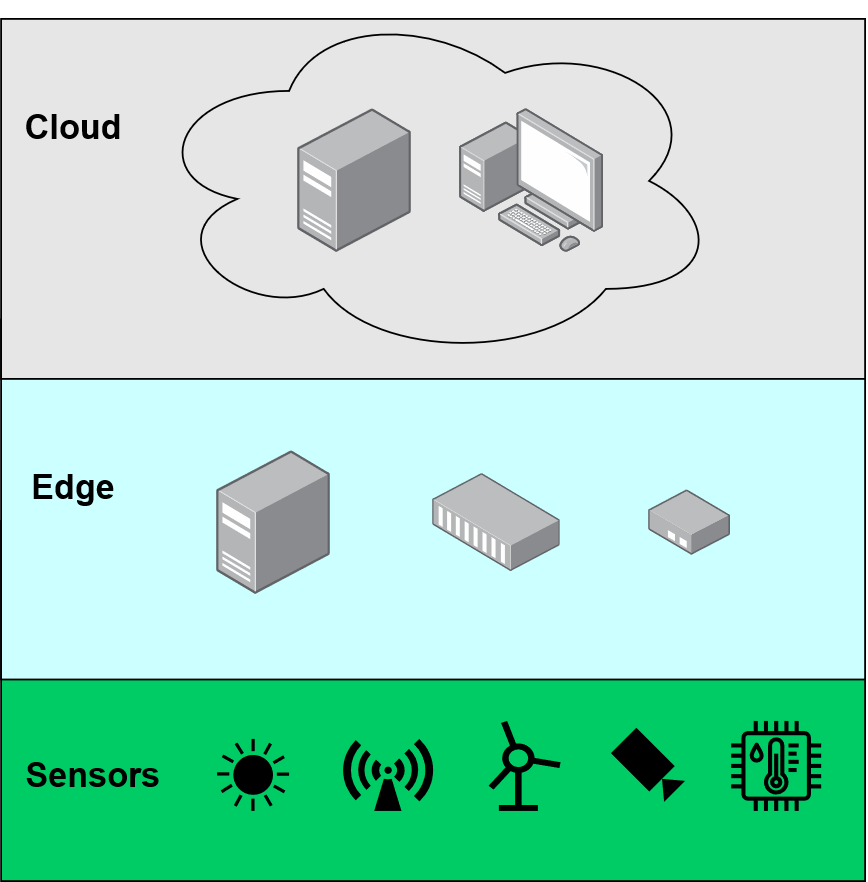
\includegraphics[width=0.8\textwidth]{imagenes/ArquitecturaCloudEdgeSensors.PNG}
  \caption{Relación entre la nube, computación de frontera y terminales}
  \label{arquitecturacloudedgesensors}
  \end{figure}
  
  A si mismo, en la Figura \ref{edgecomputinggateway} se muestra una imagen con la arquitectura de la puerta de enlace:
  
  \begin{figure}[H]
  \centering
  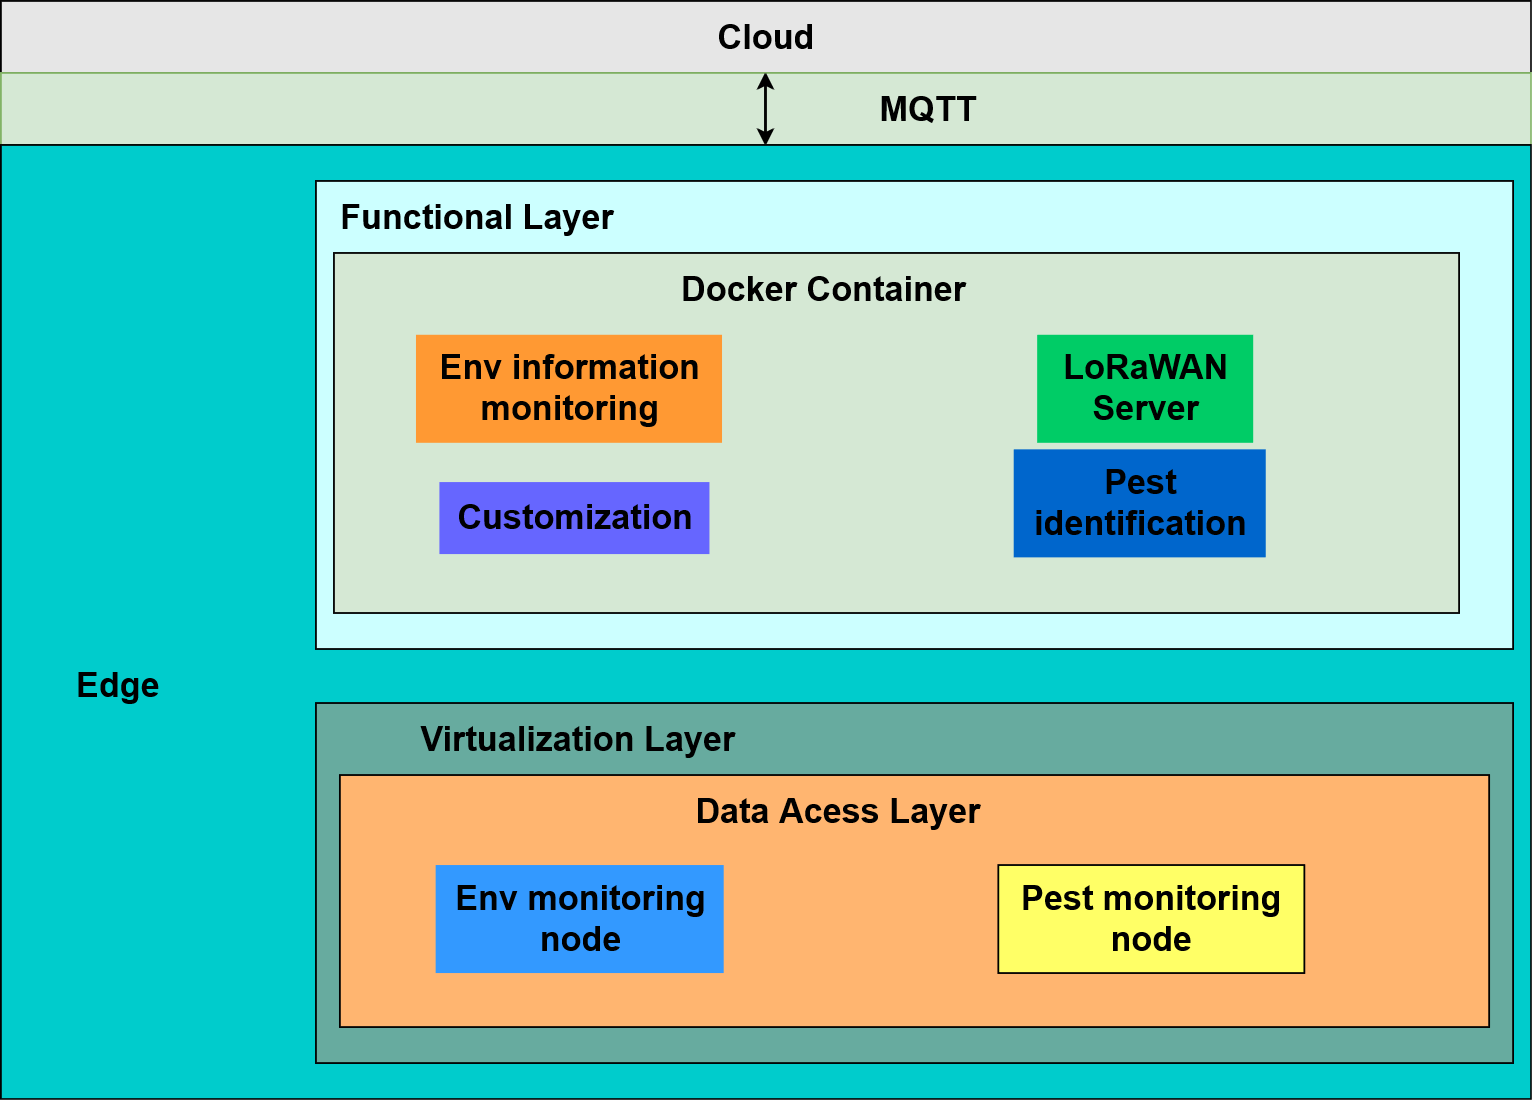
\includegraphics[width=0.8\textwidth]{imagenes/EdgeComputingGateway.PNG}
  \caption{Arquitectura de la puerta de enlace o computación de frontera}
  \label{edgecomputinggateway}
  \end{figure}
  
  \newpage

Los resultados de la investigación demostraron que \gls{Computacion de frontera} tiene la ventaja de ser de bajo costo, baja latencia y bajo consumo de poder lo que la vuelve con gran potencial para uso práctico. Así mismo el apoyo de tecnologías de contenerización y la computación en la nube vuelven al proyecto mas robusto frente a errores y la búsqueda de replicación o escalación de estas funcionalidades y se reportan terminos de reportan una tasa media de éxito en la transmisión de datos del 99,1 por ciento, con el objetivo de reducir la latencia y la carga de los servidores en la nube. 

\subsection{Evaluación experimental de sensores en un sistema de seguimiento GPS basado en LoRaWAN}

El siguiente artículo \cite{tracking_system_lora} científico se enfoca en proveer una solución basada en LoRaWAN para el desarrollo de ciudades inteligentes con el uso de sensores en
 un sistema de seguimiento GPS basado en LoRaWAN, una tecnología de comunicación inalámbrica de bajo consumo y largo alcance. 
Su objetivo es analizar el funcionamiento de los sensores y el rendimiento del sistema para la localización y transmisión de datos, 
considerando las características de esta tecnología en aplicaciones de seguimiento remoto e IoT.
El artículo resalta los beneficios de esta tecnología como es su bajo costo y poder de consumo comparado con distintas alternativas. 
A través de esta investigación el equipo de desarrollo implementa un sistema de rastreo de una flota de vehículos utilizando LoRaWAN usando como caso de estudio la ciudad de Kozani en Grecia.
La arquitectura es utilizada de la siguiente forma en la Figura \ref{applicationarchitecture}. 
Como se puede ver esta es ligeramente distinta al artículo anterior, pero cabe destacar que es bastante estándar dentro de los modelos LoRa como veremos mas adelante en el marco teórico. 

  \begin{figure}[H]
  \centering
  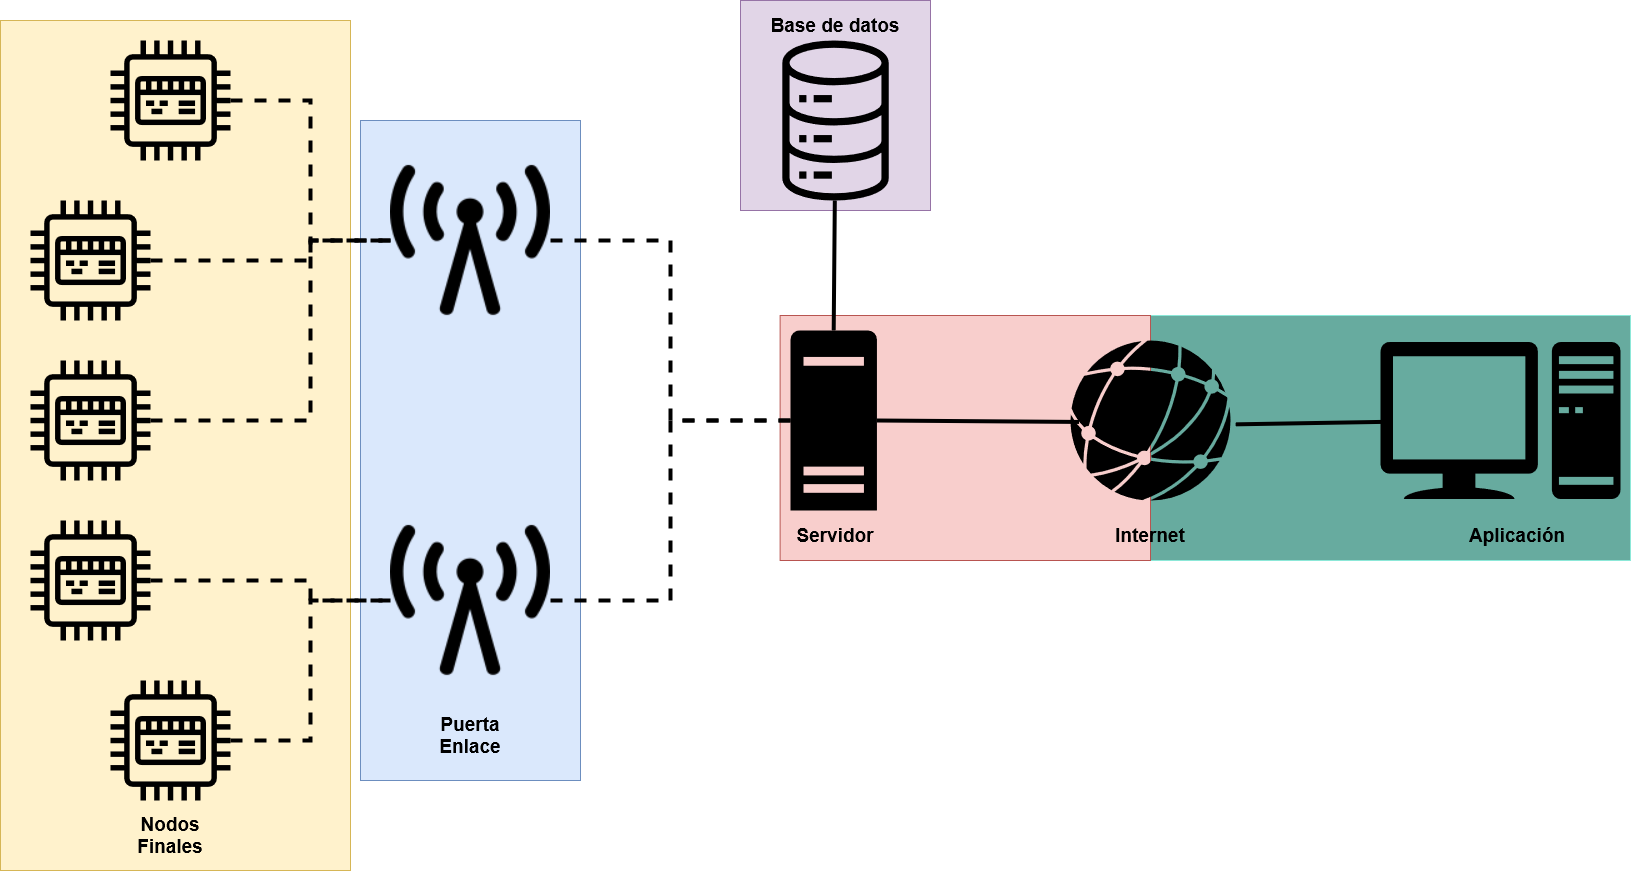
\includegraphics[width=1.1\textwidth]{imagenes/LoRaWAN-Arch.PNG}
  \caption{Arquitectura de la aplicación}
  \label{applicationarchitecture}
  \end{figure}

De izquierda a derecha la arquitectura muestra un sistema de nodos finales basados en antenas GPS comunicándose con puertas de enlace a través de LoRaWAN, estos últimos a su vez redirigen los datos a un servidor donde guardan la información en una base de datos y a través de internet llegan a una aplicación utilizando The Things Network de la cual se hablará mas adelante en el marco teórico.

\subsection{Implementación de LoRaWAN desde el dispositivo final hasta la aplicación}

Este artículo \cite{lorawan_app} habla sobre la implementación de una red completa LoRaWAN. El sistema resultante ofrece una infraestructura completa para el desarrollo de aplicaciones y
 experimentos. La red consiste en tres componentes principales. La herramienta llamada Chirpstack que es de código libre y actúa como un servidor LoRaWAN corriendo en una 
 computadora personal. La puerta de enlace LoRaWAN que es un dispositivo de red independiente y la referencia al dispositivo final que está 
 construida con componentes baratos para los autores. 

El proyecto cuenta con distintos esquemáticos ligados a través de referencias bibliográficas del dispositivo o nodo final para su fácil replicación. 
Así mismo la jerarquía utilizada para comunicar todos los dispositivos es la siguiente demostrada en la Figura \ref{fig:JerarquiaLoRaWAN} 

\begin{figure}[H]
    \centering
    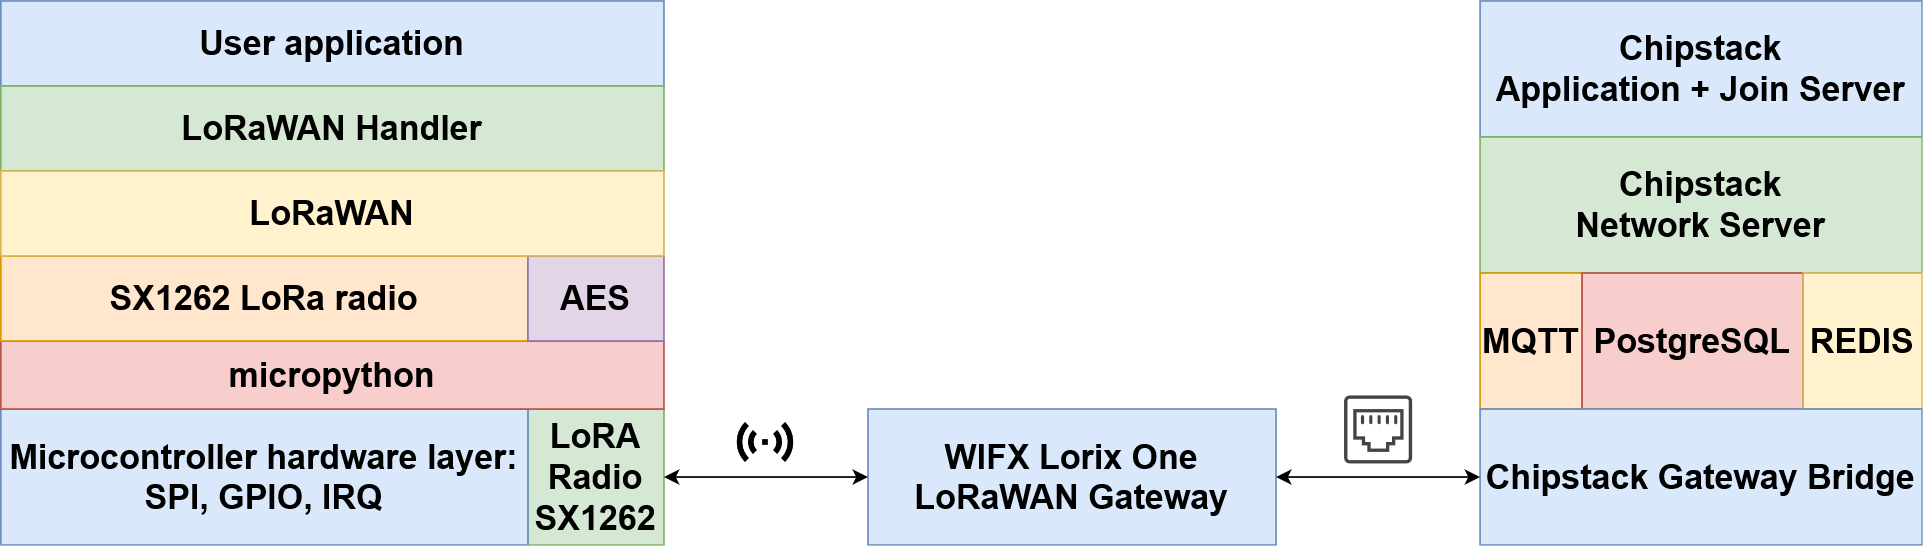
\includegraphics[width=1.0\textwidth]{imagenes/JerarquiaLoRaWAN.png}
    \caption{Jerarquía de componentes LoRa}
    \label{fig:JerarquiaLoRaWAN}
\end{figure}

Así mismo la solución propuesta por los autores esta implementada en MicroPython y se aprovecha de librerías existentes para el manejo de la tecnología y comunicación LoRaWAN.  

El servidor de red LoRaWAN está corriendo en una computadora personal aprovechando las capacidades de Docker para la generación de toda la capa de herramientas necesarias para su funcionamiento. 

Como resultados, los autores lograron obtener un servidor totalmente funcional corriendo en un contenedor que a su vez registra eventos ocurridos en el dispositivo final. 
Se hablan de las características pendientes por implementes, sin embargo, están satisfechos con el resultado debido a que la red es completamente funcional sin estas características. 

\subsection{Adquisición flexible de datos mediante LoRaWAN y MQTT para pequeñas y medianas empresas}

 Este artículo \cite{lorawan_mqtt_data_acquisition} propone una solución de LoRaWAN y MQTT para pequeñas y medianas empresas, presentando una solución generalizada para distintos tipos 
 de problemas que evade altos costos de inversión y poder obtener datos en un periodo corto de tiempo además la solución está basada en herramientas de código abierto, 
 obteniendo las ventajas de este tipo de herramientas. 
 
El enfoque propuesto es el siguiente en la Figura \ref{arquitecturaLoraGeneralPropuesta}

\begin{center}
    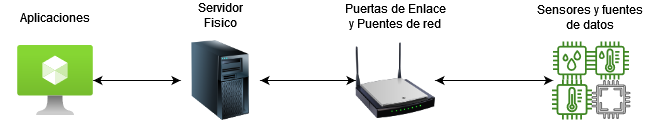
\includegraphics[width=1.0\textwidth]{imagenes/LoraWanAppProp.png}
    \captionof{figure}{Arquitectura general propuesta}
    \label{arquitecturaLoraGeneralPropuesta}
\end{center}

El artículo contribuye en proponer una solución flexible y con una infraestructura simple para la adquisición de datos a través de una red de sensores LoRaWAN y su visualización a través de una plataforma de Internet de las Cosas.

El protocolo MQTT funciona como intermediario entre LoRaWAN y la arquitectura del servidor asi como habilitador para la transferencia de datos de otras fuentes.

Asi mismo, este contribuye en aplicaciones practicas y actuales usando sensores de LoRaWAN asi como maneras de comunicarse a través de MQTT.

La solución propuesta viene de 3 componentes principales como se muestra en la Figura \ref{arquitecturaLoraGeneralPropuesta_2}:
\begin{itemize}
    \item Centro de datos
    \item Adquisición de datos con LoRaWAN
    \item Plataforma de Internet de las cosas
\end{itemize}

\begin{center}
    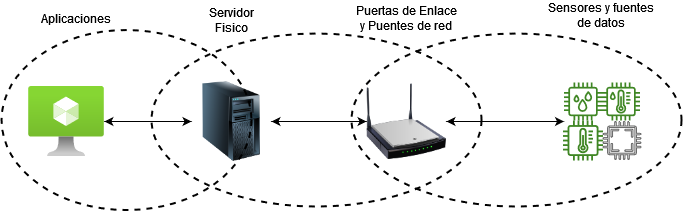
\includegraphics[width=1.0\textwidth]{imagenes/LoraWanComponentes.png}
    \captionof{figure}{Arquitectura general propuesta}
    \label{arquitecturaLoraGeneralPropuesta_2}
\end{center}


El protocolo intermediario MQTT es el centro de datos, diseñado para la conexión con dispositivos de recursos limitados. También este mismo habilita la comunicación entre 
sistemas utilizando el patrón de diseño de publicación y suscripción como se muestra en la Figura \ref{arquitecturaMQTTPropuesta}.

\begin{center}
    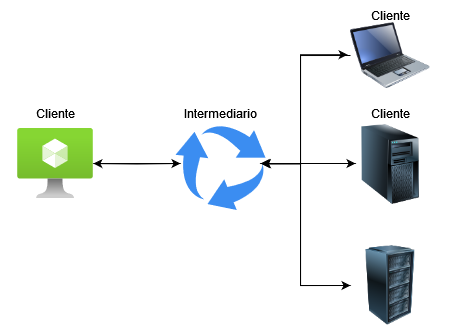
\includegraphics[width=1.0\textwidth]{imagenes/MQTTConcept.png}
    \captionof{figure}{Arquitectura MQTT propuesta}
    \label{arquitecturaMQTTPropuesta}
\end{center}


El protocolo LoRaWAN es utilizado como una red inalámbrica de sensores, proporcionando una comunicación de larga distancia.
Los sensores operados por batería son fácilmente desplegables en este tipo de protocolos y son integrados a través de una interfaz web, 
lo que hace que no sea necesario conocimientos de programación para su administración como se puede ver en la Figura \ref{arquitecturaLoRaWANPropuesta}.

\begin{center}
    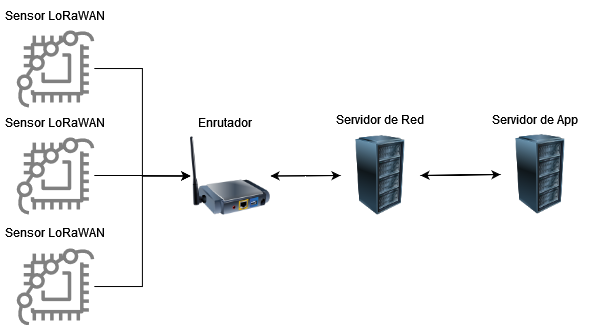
\includegraphics[width=1.0\textwidth]{imagenes/LoRaWANConcept.png}
    \captionof{figure}{Arquitectura LoRa propuesta}
    \label{arquitecturaLoRaWANPropuesta}
\end{center}


La plataforma IoT es desplegada como se ve en la Figura \ref{arquitecturaIoTPropuesta} y utilizada para medir los datos obtenidos en un panel web. Esto propicia a una visualización y medición con poco esfuerzo, 
además de permitir agregar otras fuentes de datos gracias a su integración con MQTT

\begin{center}
    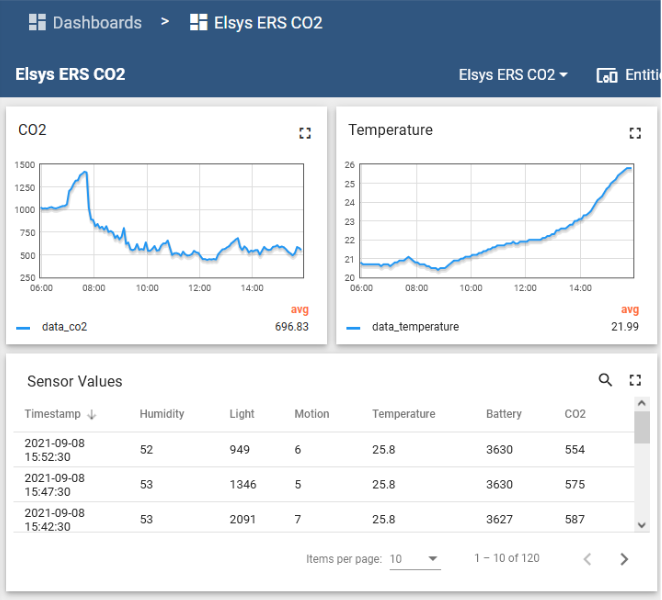
\includegraphics[width=1.0\textwidth]{imagenes/PlataformaIoT.png}
    \captionof{figure}{Plataforma IoT propuesta}
    \label{arquitecturaIoTPropuesta}
\end{center}

El sistema implementado puede gestionar aproximadamente 5.000 mensajes MQTT por segundo con cargas útiles inferiores a 1.000 bytes, según la evaluación de rendimiento 
presentada por los autores.
En conclusión, este trabajo demuestra el conjunto de herramientas en un solo proyecto con múltiples tipos de aplicación, el cual definitivamente es una buena base para 
el presente proyecto.

\subsection{Diseño de una pasarela LoRaWAN con servidores autónomos para comunidades sin conexión a Internet}

Este artículo \cite{local_things_network} habla de como los dispositivos IoT en la práctica deberían ser sencillos de desplegar asi como deberían durar activos 
largos periodos en campo sin ninguna intervención. Se propone el uso del protocolo LoRaWAN para conseguir estos objetivos, además, se habla del uso de un conjunto de 
herramientas llamado The Things Networks el cual en Europa es fácilmente accesible ya que cuenta con dispositivos usables en campo para conectar con dispositivos LoRaWAN finales.

Debido a que no se puede garantizar siempre tener internet en muchos países, se propone una solución utilizando nodos IoT locales a una puerta de enlace LoRaWAN sin la 
necesidad de emplear redes de internet, a un bajo costo y poco poder de consumo. 

Los investigadores implementaron tres bloques de la arquitectura LoRaWAN (Puerta de enlace, Servidor de Red, Servidor de Aplicación) en un solo dispositivo utilizando una Raspberry Pi 
y un modulo LoRaWAN. 
El acceso local a los datos de la aplicación es a través de un punto de acceso WiFi, permitiendo a los miembros de la comunidad acceder a sus datos comunitarios incluso cuando no hay 
internet. Además de datos IoT en tiempo real, los investigadores proponen servicios extra que pueden ser implementados en el repositorio para ayudar en el desarrollo de la educación, 
salud y otros contenidos que pueden apoyar a comunidades distantes. 

\begin{center}
    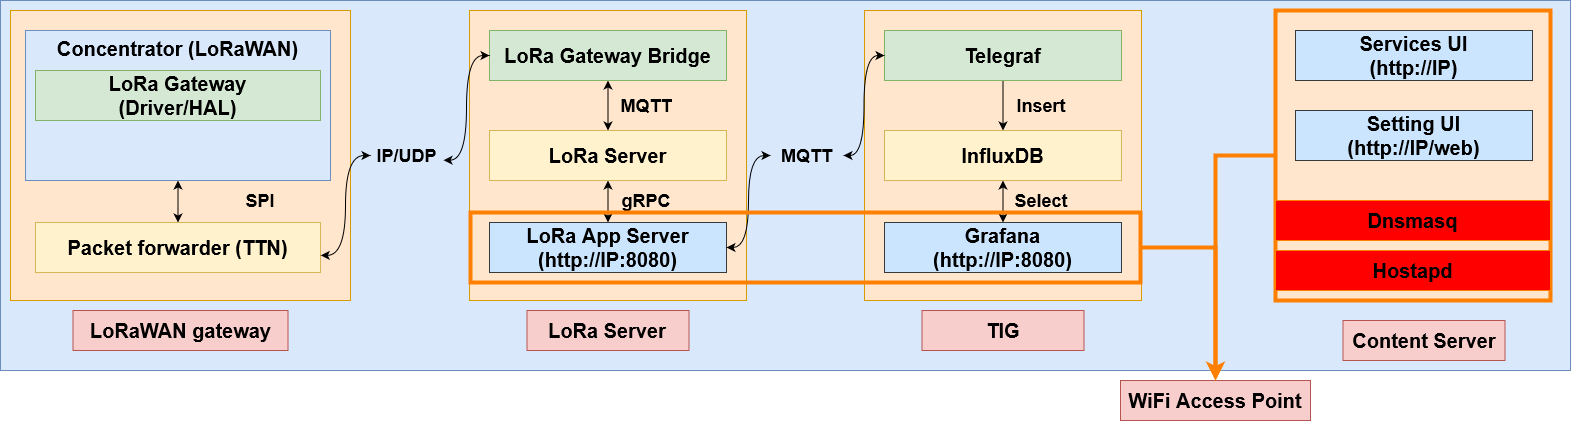
\includegraphics[width=1.0\textwidth]{imagenes/PartsOfBS.png}
    \captionof{figure}{Partes de una Estación Base}
    \label{PartsOfBaseStation}
\end{center}

El dispositivo completo con todas estas características es llamado la Estación Base (BS en inglés).
La arquitectura de la estación base es dividida en cuatro partes como se muestra en la Figura \ref{PartsOfBaseStation}: Puerta de enlace LoRaWAN (GW en inglés), Servidor de aplicación y de red, un componente llamado TIG (De las siglas Telegraf, InfluxDB y Grafana), el punto de acceso WiFi y el servidor de contenido

Puerta de Enlace LoRaWAN Figure \ref{BSwith8and1channel}. Actúa como un transmisor de paquetes entre un nodo final y un servidor de red basado en la implementación de código abierto propuesta por Semtech y 
construida en una Raspberry Pi. El equipo de investigadores cuenta con dos versiones, la más robusta que usa un módulo SX1301 la cual admite comunicación simultanea mientras escucha en ocho diferentes frecuencias y la mas barata utilizando un módulo RFM96W el cual solo admite un solo canal.

Servidor de red y servidor de aplicación. El rol del servidor de red es autenticar nodos y estar seguro de que solo se reciben datos de los dispositivos registrados. 
El servidor de aplicación provee procesamiento de tramas y su desencriptación. Asi mismo, ofrece al usuario final los datos solicitados, como el clima, la calidad del aire, alarmas, etc.
 Los datos son localmente procesados, guardados y se pueden accesar a través del punto de entrada WiFi 

TIG. La herramienta de Telegraf es usada para suscribirse a un intermediario de mensajes MQTT y recolectar mensajes en formato JSON los cuales son transmitidos por el servidor de
 aplicación LoRa y esto se inyectan en InfluxDB una base de datos de series de tiempo (TSDB en inglés). Gracias a Grafana (Una plataforma de código abierto para gráfico de datos) las mediciones pueden ser obtenidas de InfluxDB para su análisis y monitoreo.

Servidor de Contenido. El servidor de contenido provee acceso al contenido estático, como el material educacional, información de salud, las mejores prácticas de agricultura, etc. 
Asi como un tablero que funciona como boletín de información para la comunidad. El punto de acceso WiFi hace este material disponible a través de la comunidad usando una interfaz web. 

\begin{center}
    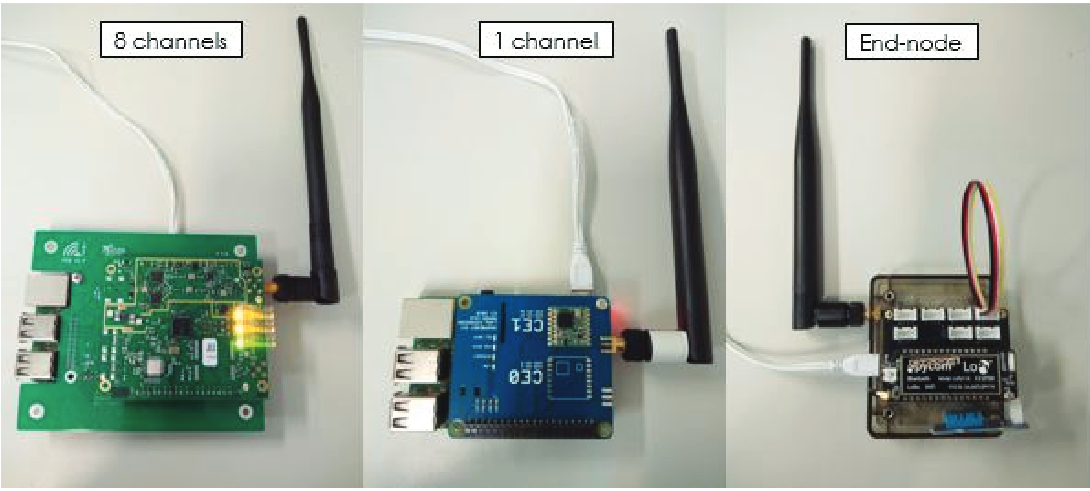
\includegraphics[width=1.0\textwidth]{imagenes/NodosPaper3.png}
    \captionof{figure}{BS con 8 canales (izquierda), 1 canal (centro) y un nodo final (derecha).}
    \label{BSwith8and1channel}
\end{center}

En conclusión, este trabajo está enfocado a extender los beneficios de utilizar IoT en personas que viven en áreas con muy limitado o sin acceso a conexiones de internet, utilizando redes y servidores LoRaWAN los cuales pueden ser encapsulados en dispositivos pequeños que proveen todas las funcionalidades requeridas. Asi mismo pueden tomar ventaja de dispositivos TTN si es que están disponibles, de forma intermitente, incluso pueden ser soluciones independientes que sirvan a una comunidad. Los usuarios pueden interactuar con el BS propuesto utilizando sus dispositivos propios a través de la conexión WiFi.
El trabajo futuro de los investigadores se centrará en el tablón de anuncios y el contenido sistemas de gestión que son características muy útiles para comunidades aisladas, así como en una extensión de este modelo al acomodar la sincronización de la base de datos de varias BS desplegadas en la misma comunidad, interconectadas entre sí pero independientes de una conexión a Internet.

\subsection{Particionado de red de acceso radio en redes LoRaWAN}

En el siguiente trabajo de final de grado \cite{particionado_de_red_lorawan} vemos que en este se propone dividir los recursos de una red LoRaWAN en segmentos o 
\textit{slices}, que puedan asignarse a distintos usuarios o proveedores. Para ello, define un bloque de recursos (RB) como la combinación de un canal y un 
factor de dispersión (SF). En la configuración estudiada, los ocho canales de 125 kHz y los SF del 7 al 12 permiten formar hasta 48 combinaciones de recursos.

La solución se implementa sobre una red LoRaWAN con ChirpStack y dispositivos reales. El servidor asocia cada dispositivo con un \textit{slice} y, durante el 
intercambio de mensajes de unión, envía al dispositivo una máscara que indica los RB disponibles. A partir de esa máscara, el dispositivo selecciona un RB y 
configura el canal y el SF de transmisión según las condiciones de la señal, estimadas mediante el indicador de fuerza de señal recibida (RSSI) o la relación 
señal-ruido (SNR). Así, la selección del SF puede ajustarse a la calidad del enlace, mientras que la separación por canal y SF permite organizar las transmisiones 
de distintos usuarios.

La arquitectura utilizada para implementar esta solución se resume en la Figura \ref{arquitecturaParticionadoLoRaWAN}. Las micro tarjetas o como el autor se refiere 
motas de modelo LoPy4 se comunican con la pasarela mediante LoRaWAN, y esta reenvía los paquetes al servidor, donde ChirpStack y el sistema de 
particionado gestionan la asignación de recursos.

\begin{center}
    \begingroup
    \shorthandoff{<>}
    \begin{tikzpicture}[font=\small]
        \node[draw, rounded corners, align=center, text width=8cm, minimum height=1.5cm]
            (motas) at (0,0) {\textbf{Dispositivos finales}\\Motas LoPy4};

        \node[draw, rounded corners, align=center, text width=8cm, minimum height=1.5cm]
            (gateway) at (0,-2.5) {\textbf{Pasarela LoRaWAN}\\PyGate LoPy con escudo};

        \draw[<->, thick] (motas.south) -- node[midway, xshift=1cm, anchor=west, align=left]
            {\scriptsize LoRaWAN: \texttt{JOINREQ} / \texttt{JOINACC}} (gateway.north);

        \node[draw, rounded corners, minimum width=14.2cm, minimum height=4.8cm]
            (servidor) at (0,-7.2) {};
        \node[align=center] at (0,-5.2)
            {\textbf{Servidor LoRaWAN en Raspberry Pi 4}};

        \node[draw, rounded corners, align=center, text width=4cm, minimum height=1.5cm]
            at (-4.6,-6.45) {\textbf{Gateway Bridge}\\Reenvío y formato};
        \node[draw, rounded corners, align=center, text width=4cm, minimum height=1.5cm]
            at (0,-6.45) {\textbf{Servidor de red}\\Gestión de la red};
        \node[draw, rounded corners, align=center, text width=4cm, minimum height=1.5cm]
            at (4.6,-6.45) {\textbf{Aplicación}\\Gestión de dispositivos};
        \node[draw, rounded corners, align=center, text width=12.8cm, minimum height=1.5cm]
            at (0,-8.45) {Broker MQTT, algoritmo de particionado\\y base de datos de dispositivos y \textit{slices}};

        \draw[<->, thick] (gateway.south) -- node[midway, xshift=1cm, anchor=west, align=left]
            {\scriptsize IP: reenvío de paquetes} (servidor.north);
    \end{tikzpicture}%
    \endgroup
    \captionof{figure}{Arquitectura utilizada para el particionado de la red LoRaWAN}
    \label{arquitecturaParticionadoLoRaWAN}
\end{center}

Las pruebas confirmaron la comunicación entre los dispositivos y el servidor, así como la asignación de recursos según el SNR. En particular, las simulaciones 
mostraron que, para los valores de SNR evaluados, el algoritmo no asignaba factores de dispersión incompatibles con la calidad de la señal. En cambio, no fue posible 
validar el algoritmo basado en RSSI, pues durante las pruebas no se alcanzaron condiciones de cobertura suficientes para que funcionara. El trabajo concluye que el 
particionado propuesto es viable en LoRaWAN y plantea como líneas futuras ampliar los criterios de selección, analizar el rendimiento y el consumo energético, y permitir 
que el usuario elija el \textit{slice} según los requisitos de calidad de servicio.

\subsection{Diseño de un Nodo LoRa-GPS para Localización de Bicicletas Implementado en una Red LoRaWAN}

El trabajo de fin de grado de Jairo Andrés Rodríguez Sánchez y Jhoiner Smith Rojas González \cite{nodo_lora_gps} aborda el diseño de un nodo para 
localizar bicicletas mediante la integración de posicionamiento GPS y comunicación LoRaWAN. A nivel funcional, el nodo obtiene las coordenadas de la 
bicicleta y las transmite a través de la red para que puedan ser recibidas y consultadas por el usuario. Este enfoque aprovecha el alcance de LoRaWAN 
para comunicar un dispositivo móvil con una aplicación de seguimiento.

La Figura \ref{arquitecturaNodoLoRaGPS} presenta un esquema general del flujo de información: desde la obtención de la posición en la bicicleta hasta 
su consulta en la aplicación. Se muestran los componentes funcionales de una arquitectura LoRaWAN, sin especificar modelos de hardware ni plataformas 
de software particulares.

\begin{center}
    \begingroup
    \shorthandoff{<>}
    \begin{tikzpicture}[font=\small]
        \node[draw, rounded corners, align=center, text width=8.5cm, minimum height=1.5cm]
            (bicicleta) at (0,0)
            {\textbf{Bicicleta}\\Nodo LoRa-GPS: obtiene las coordenadas};

        \node[draw, rounded corners, align=center, text width=8.5cm, minimum height=1.5cm]
            (gateway) at (0,-2.3)
            {\textbf{Pasarela LoRaWAN}\\Recibe los mensajes del nodo};

        \draw[->, thick] (bicicleta.south) -- node[midway, xshift=1cm, anchor=west]
            {\scriptsize LoRaWAN} (gateway.north);

        \node[draw, rounded corners, align=center, text width=10cm, minimum height=1.5cm]
            (servidor) at (0,-4.6)
            {\textbf{Servidor LoRaWAN}\\Recibe y entrega los datos de posición a la aplicación};

        \draw[->, thick] (gateway.south) -- node[midway, xshift=1cm, anchor=west]
            {\scriptsize Conexión IP} (servidor.north);

        \node[draw, rounded corners, align=center, text width=8.5cm, minimum height=1.5cm]
            (aplicacion) at (0,-6.9)
            {\textbf{Aplicación de seguimiento}\\Presenta al usuario la ubicación de la bicicleta};

        \draw[->, thick] (servidor.south) -- node[midway, xshift=1cm, anchor=west]
            {\scriptsize Datos de posición} (aplicacion.north);
    \end{tikzpicture}%
    \endgroup
    \captionof{figure}{Esquema funcional general de localización de bicicletas con LoRaWAN}
    \label{arquitecturaNodoLoRaGPS}
\end{center}

\section{Marco teórico}

\subsection{LoRa y LoRaWAN}

LoRa es una especificación de una red LPWAN propuesta por LoRa Alliance \cite{lorawan_definition} y pensada para comunicar dispositivos de bajo costo y bajo 
consumo de energía alimentados por baterías. La especificación cubre la capa física y la de acceso al medio de la red, dejando a las aplicaciones el resto de las capas. 
La comunicación entre los dispositivos y las puertas de enlace (nombradas gateways por la especificación en inglés) se basa en la modulación LoRa desarrollada por la compañía 
Semtech \cite{semtech_lora}. Esta modulación permite enlaces de varios kilómetros inclusive en entornos urbanos, gracias a su presupuesto de enlace máximo de 155 dB, 
con una tasa de bit entre 0.3 kbps y 50 kbps. En cuanto a las particularidades de la modulación LoRa, diferentes dispositivos emitiendo en la misma frecuencia, 
pero con tasa de bit distinta, no corrompen las transmisiones. Esto permite disponer de un amplio número de canales virtuales para la comunicación entre dispositivos finales y 
estación base. En la siguiente Figura \ref{fig:ArquitecturaLoRa} se muestra la pila de protocolos que utiliza LoRa.

\begin{figure}[H]
    \centering
    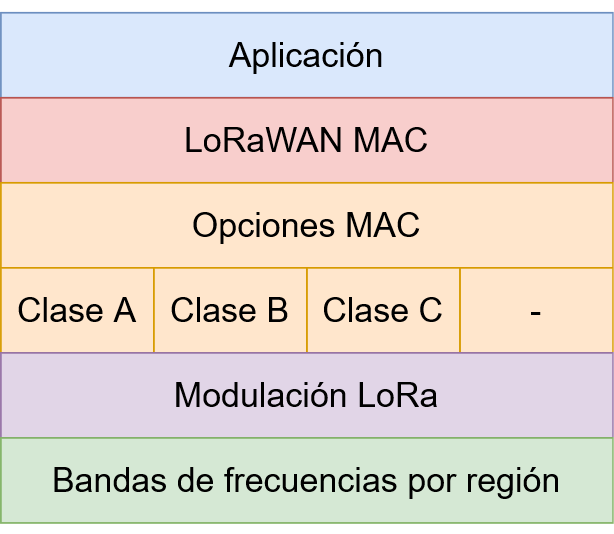
\includegraphics[width=1.0\textwidth]{imagenes/ArquitecturaLoRa.png}
    \caption{Arquitectura LoRa}
    \label{fig:ArquitecturaLoRa}
\end{figure}

\newpage

La topología de red propuesta por LoRaWAN es estrella, es decir, los dispositivos finales se comunican directamente a un salto 
con una estación base de forma bidireccional. Las estaciones base transmiten los datos de los dispositivos finales al servidor de red y viceversa 
utilizando una conexión IP estándar. En la Figura \ref{fig:LoRaWANTopologia} se muestra la arquitectura utilizada en redes LoRa.

\begin{figure}[H]
    \centering
    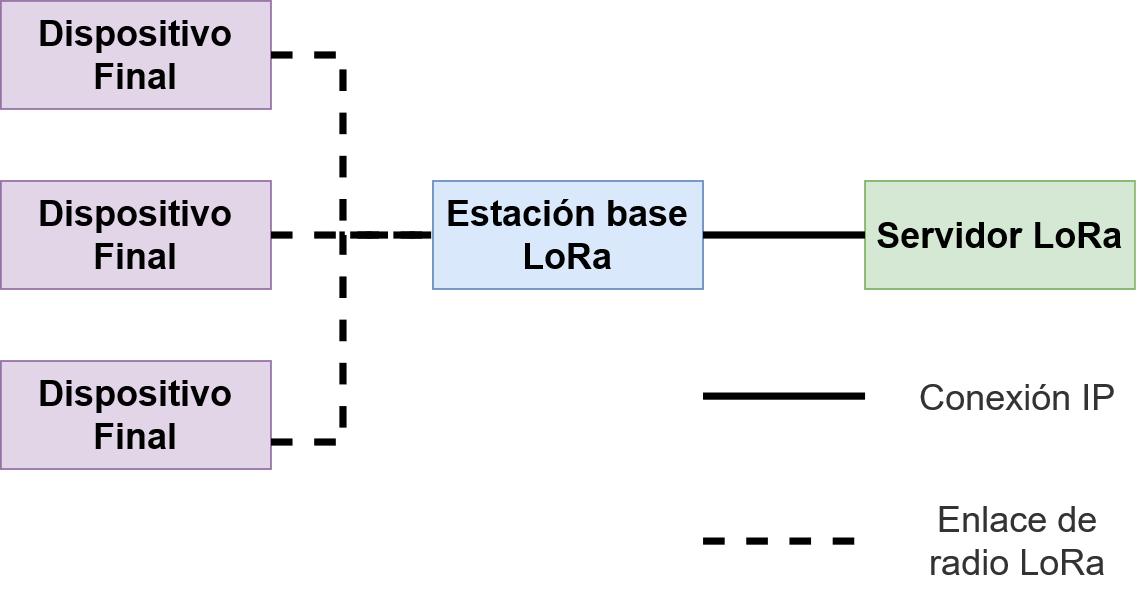
\includegraphics[width=1.0\textwidth]{imagenes/LoRaWANTopologia.png}
    \caption{Topología LoRa}
    \label{fig:LoRaWANTopologia}
\end{figure}

\subsection{Docker}

\gls{Docker} es un motor de contenedores de código libre que utiliza una virtualización\cite{docker_definition} ligera permitiendo automatizar el despliegue de 
aplicaciones mediante \gls{Contenedor} virtuales. Esto significa que puede encapsular las aplicaciones dentro de un contenedor junto con sus dependencias y ejecutarlos sobre 
cualquier equipo que tenga instalada la plataforma \gls{Docker}, usualmente servidores Linux, nubes públicas y privadas. \gls{Docker} amplía LXC con un kernel y una Interfaz de 
Programación de Aplicaciones (API, por sus siglas en inglés) a nivel de aplicación que permiten la ejecución de procesos aislando CPU, memoria, E/S, red, etc. Además, 
Docker utiliza diferentes espacios de nombre para aislar por completo la vista de una aplicación del entorno subyacente (sistema operativo), lo que incluye los árboles de 
procesos, la red, los IDs de usuario y los sistemas de archivos

\subsection{The Things Network}

The Things Network (TTN), es una red de IoT global, descentralizada, gratuita, abierta y en la que cualquier persona puede aportar sus conocimientos acerca de IoT con la finalidad 
de mejorar cada vez más la plataforma. TTN fue creado en el verano de 2015 en Amsterdam, por sus dos fundadores Wienke Giezeman y Johan Stokking\cite{the_things_network_definition}, 
entre otros y cuyo objetivo era facilitar el diseño y la creación de redes, para lo cual daba soporte a las distintas puertas de enlace distribuidos por el mundo y además ofrecía la 
infraestructura de back-end a sus usuarios, es decir, una implementación de las funcionalidades del servidor de red y del servidor de aplicación. 

Este set de herramientas del lado del servidor se enfrenta a duplicidades de mensajes, gestiona la transmisión de mensajes descendentes, gestiona integraciones con plataformas, 
como HTTP o MQTT y ofrece una serie de APIs en diferentes lenguajes de programación como Java, Node.js o Node-Red. 

Como se trata de una plataforma código abierto, los códigos con los que se ha construido el set de herramientas del lado del servidor son públicos y se puede acceder a ellos a 
través de un proyecto en GitHub. Actualmente TTN tiene registradas alrededor de 9000 puertas de enlace distribuidos por todo el mundo y están registrados más de 80000 miembros. 

Teniendo en cuenta que hace tan solo un año había registradas 3000 puertas de enlace, se puede pensar que  la idea de la evolución tan rápida que está teniendo la tecnología 
LoRaWAN y a su vez la red de TTN. En la siguiente Figura \ref{fig:TheThingsStackMap} se puede observar la distribución de las puertas de enlace en el mundo: Este continuo crecimiento de la comunidad permite 
a muchas personas acceder de manera muy sencilla y gratuita a un entorno IoT donde poder realizar proyectos o implementar sus ideas.

\begin{figure}[H]
    \centering
    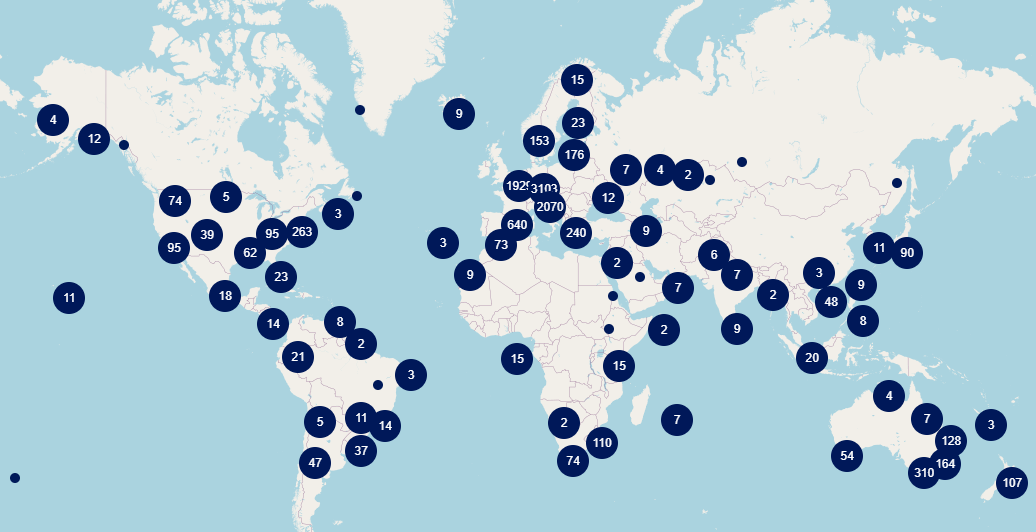
\includegraphics[width=1.0\textwidth]{imagenes/TheThingsStackMap.PNG}
    \caption{Mapa con la distribución de las puertas de enlace en el mundo para The Things Network}
    \label{fig:TheThingsStackMap}
\end{figure}

Además, TTN ha desarrollado una gran cantidad de comunidades en las que los usuarios, generalmente ubicados en las mismas zonas geográficas puedan intercambiar información o 
conocimientos que puedan ser útiles para otros usuarios y así, de manera recíproca pueden servirse de ayuda unos con otros. Por ejemplo, en España se han creado recientemente 
varias comunidades de TTN en Mexico, Estados Unidos, Países en Suramérica, etc., lo cual indica que se está notando el auge de LoRaWAN de forma más cercana.
    % Capitulo 02

        \chapter{Metodología}
        %Capítulo 3

\section{Diseño del servidor LoRa}
    
    \textbf{\textit{Descripción}}
    
 Como se explicó en el capitulo anterior es necesario un conjunto de tecnologías distintas para lograr nuestro propósito de generar un servidor que administre los distintos nodos. En la siguiente sección se explica con mas detalle toda la arquitectura propuesta para la implementación del servidor maestro. 
\\
\\El objetivo es desarrollar todo un ecosistema IoT completo que sea lo suficientemente genérico para poder ser soportado y redesplegado en distintos proyectos, pero al mismo tiempo lo suficientemente especializado para cumplir las funciones de administrar los nodos asi como su manejo de la información.
\section{Diseño de arquitectura implementado}
    \textbf{\textit{Diagrama de arquitectura}}

Tras la investigación del estado del arte decidí implementar la siguiente arquitectura de configuración basándome en el estado del arte de proyectos anteriores. Por lo que encontraran bastante similitud con los mismos, aunque por supuesto con diferencias específicas para apoyar al equipo de investigadores que usaran el sistema. En la Figura \ref{fig:arquitectura-implementada} se muestra el diagrama final.

\begin{figure}[H]
    \centering
    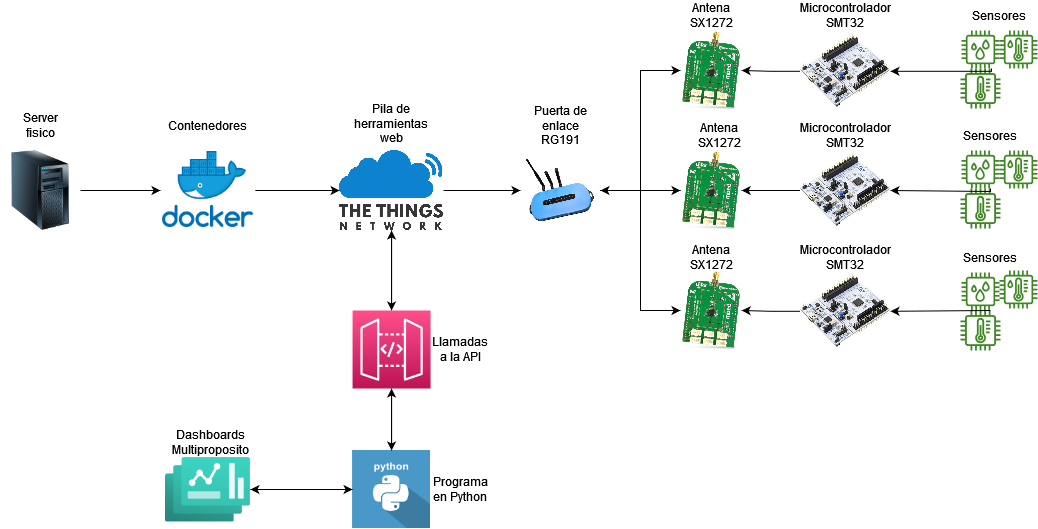
\includegraphics[width=1.0\textwidth]{imagenes/LoraWanUAGArch.png}
    \caption{Arquitectura implementada para el sistema de nodos}
    \label{fig:arquitectura-implementada}
\end{figure}

El servidor físico cuenta con una instancia de Docker para facilitar su portabilidad a otros sistemas distintos o inclusive su montaje en la nube. Dentro del contenedor se encuentra instalado The Things Stack el cual nos facilita la comunicación con múltiples puertas de enlace de tipo RG191 asi como con la administración de los nodos LoRa que funcionan atraves del microcontrolador SMT32 con su antena SX1272.
A continuación, explicare todos los pasos necesarios para la configuración y lanzamiento de un servidor.  

\section{Configuración del servidor LoRa}
 \subsection{Prerrequisitos}

Primeramente, debemos tener configurado nuestro entorno donde todo el sistema vivirá. Para este caso de uso utilizamos una distribución Debian. Para instalarlo podemos utilizar la \gls{guiadebian} proporcionada por Debian, sin embargo, tal y como explique antes. El sistema puede ser montado en cualquier sistema operativo o inclusive en la nube. 

\subsection{Instalación de Docker}

Una vez que tengamos una distribución de Linux en funcionamiento, debemos instalar Docker.Para mayor comodidad Debian ya proporciona una \href{https://docs.docker.com/engine/install/debian/}{guía de como instalar Docker} de forma sencilla en su distribución

Una vez instalado Docker podemos probar la instalación:

\begin{lstlisting}
    sudo docker run hello-world
\end{lstlisting}

Ahora, con docker instalado, podemos instalar docker-compose para facilitar la gestión de diferentes contenedores.

La forma más fácil de instalar es verificar la última versión aquí y descargar los archivos binarios más recientes usando el comando curl:

\begin{lstlisting}
   sudo curl -L https://github.com/docker/compose/releases/
   download/1.25.3/docker-compose-`uname -s`-`uname -m` 
   -o /usr/local/bin/docker-compose
\end{lstlisting}

A continuación, debemos configurar los permisos.

\begin{lstlisting}
    sudo chmod +x /usr/local/bin/docker-compose
\end{lstlisting}
    
Finalmente, solo verifique que esté funcionando

\begin{lstlisting}
    docker-compose --version
\end{lstlisting}
    

\subsection{Instalación de The Things Stack}

El siguiente paso para crear una instalación limpia es descargar los archivos de The Things Stack la cual como se explico anteriormente es la suite utilizada para el manejo de los dispositivos LoRa.
Lo primero que debemos hacer es crear una estructura de carpetas con los siguientes comandos:

\begin{lstlisting}
    mkdir the-things-stack
    mkdir config
    mkdir config/stack
\end{lstlisting}

Descargar los archivos necesarios y cámbiarle el nombre para que se pueda utilizar en Docker

\begin{lstlisting}
    curl https://www.thethingsindustries.com/docs/
    getting-started/installation/configuration/
    docker-compose-open-source.yml > docker-compose.yml
    
    curl https://www.thethingsindustries.com/docs/
    getting-started/installation/configuration/
    ttn-lw-stack-docker-open-source.yml > ttn-lw-stack-docker.yml
\end{lstlisting}

Modifique los archivos para satisfacer sus necesidades. Recuerde que puede usar archivos en el \href{https://github.com/francofonseca/lorawan_gateway}{repositorio} como ejemplo o seguir la guía de configuración oficial.

Descargar las imágenes de dockerfile

\begin{lstlisting}
    sudo docker-compose pull
\end{lstlisting}

Ahora tenemos las imágenes listas para usar.

\subsection{Configuración de certificados}

Antes de que podamos continuar configurando las imágenes de Docker, debemos asegurarnos de que podremos conectarnos a nuestro panel web sin problemas, para hacer esto, necesitamos configurar algunos certificados.

En el repositorio ya están los certificados necesarios para realizar esta tarea, en caso de que quieras crear tus certificados desde cero puedes seguir la \href{https://www.thethingsindustries.com/docs/getting-started/installation/certificates/}{guía de configuración oficial}

Para generar certificados, necesitaremos herramientas cfssl. Esta herramienta está construida con el lenguaje de programación Go, por lo que, para empezar, debemos descargar la \href{https://go.dev/dl/}{versión más reciente de la página web de Go}.

Antes de que podamos continuar configurando las imágenes de nuestra ventana acoplable, debemos asegurarnos de que podremos conectarnos a nuestro tablero sin problemas, para hacer esto, necesitamos configurar algunos certificados.

En el repositorio ya están los certificados necesarios para realizar esta tarea, en caso de que quieras crear tus certificados desde cero puedes seguir la guía de configuración oficial

Despues:

\begin{lstlisting}
    #Descomprimir Go
    tar -xzf go1.19.4.linux-amd64.tar.gz

    #Mover GO a la carpeta local
    sudo mv go /usr/local/

    #Configurar GOROOT env var
    export GOROOT=/usr/local/go

    #Verificar instalacion
    go --version
\end{lstlisting}


Ahora, con Go ejecutándose, necesitamos descargar las herramientas de cfssl. Podemos hacerlo desde el repositorio de cfssl.

\begin{lstlisting}
    git clone https://github.com/cloudflare/cfssl.git

    #Moverse dentro de la carpeta generada
    cd cfssl

    #Construir el repositorio
    make
\end{lstlisting}

Una vez que los pasos sean exitosos, se creará una carpeta bin, agregue esta ruta a la variable de entorno PATH como esta

\begin{lstlisting}
    export PATH="/home/uaguser/Downloads/cfssl/bin:$PATH"
\end{lstlisting}

Ahora necesitamos crear el archivo de certificado llamado ca.json con el siguiente contenido

\begin{lstlisting}
    {
        "names": [
            {
                "C": "NL", 
                "ST": "Noord-Holland", 
                "L": "Amsterdam", 
                "O": "The Things Demo"
            }
        ]
    }
\end{lstlisting}

Este es un ejemplo de los datos que puede modificar a su gusto siguiendo las reglas del certificado
Luego ejecute lo siguiente para generar la clave y el certificado de CA

\begin{lstlisting}
    cfssl gencert -ca ca.pem -ca-key ca-key.pem cert.json | cfssljson -bare cert
\end{lstlisting}

Ahora escriba la configuración de su certificado en cert.json

\begin{lstlisting}
    {
        "hosts": ["thethings.example.com"],
        "names": [
            {
                "C": "NL", 
                "ST": "Noord-Holland", 
                "L": "Amsterdam", 
                "O": "The Things Demo"}
        ]
    }
\end{lstlisting}

Ejecute el siguiente comando para generar la clave del servidor y el certificado

\begin{lstlisting}
    cfssl gencert -ca ca.pem -ca-key ca-key.pem 
    cert.json | cfssljson -bare cert
\end{lstlisting}


Ahora cambie el nombre de su certificado cert-key.pem a key.pem

\begin{lstlisting}
    mv cert-key.pem key.pem
\end{lstlisting}

Debian solo reconoce certificados en formato crt, por lo que es hora de convertir ambos certificados

\begin{lstlisting}
    openssl x509 -outform der -in ca.pem -out ca.crt
    openssl x509 -outform der -in cert.pem -out cert.crt
\end{lstlisting}

Copie su certificado en la carpeta de certificados, esto puede ser diferente según su distribución de Linux

\begin{lstlisting}
    sudo cp ca.crt /usr/local/share/ca-certificates/
\end{lstlisting}

Cambie los permisos de sus certificados

\begin{lstlisting}
    sudo chmod 600 /usr/local/share/ca-certificates/ca.*
    chmod 777 ca.pem 
    chmod 777 cert.pem 
    chmod 777 key.pem 
\end{lstlisting}

Actualice sus certificados

\begin{lstlisting}
    sudo update-ca-certificates
\end{lstlisting}

Su árbol de archivos ahora debería verse así, excluyendo la carpeta blob

\begin{figure}[H]
    \centering
    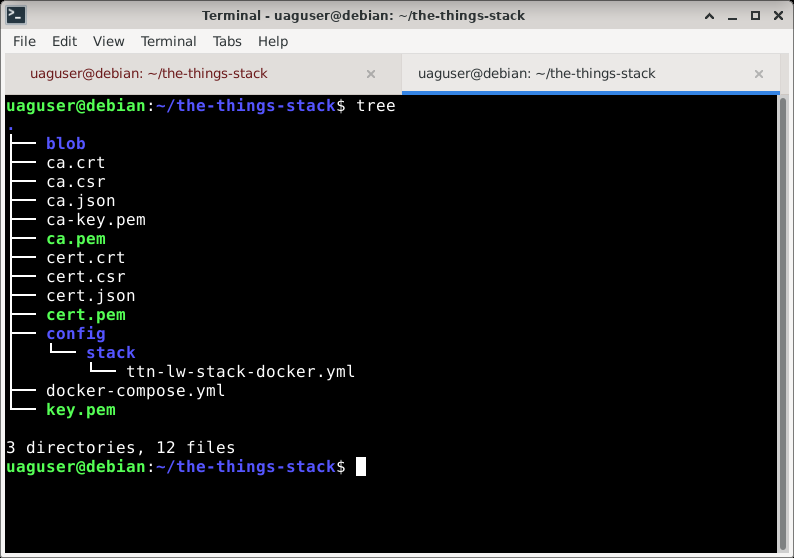
\includegraphics[width=1.0\textwidth]{imagenes/imagenes_manual/treeoffiles.png}
    \caption{Árbol de archivos}
    \label{fig:arbol-de-archivos}
\end{figure}

\subsection{Configurar LAIRD Sentrius RG191}

Ahora que configuramos los certificados, estamos listos para configurar nuestro Laird Gateway y las IP del servidor para comunicarnos.

Primero, debemos acceder a la puerta de enlace de Laird para hacerlo, consulte el \href{https://assets.lairdtech.com/home/brandworld/files/Sentrius%20RG1xx%20User%20Guide%20v2_2.pdf}{capítulo 4 de la documentación oficial} \textit{Inicie sesión en la puerta de enlace}.

Deberíamos ver algo como en la Figura \ref{fig:rg191-pagina-principal}.

\begin{figure}[H]
    \centering
    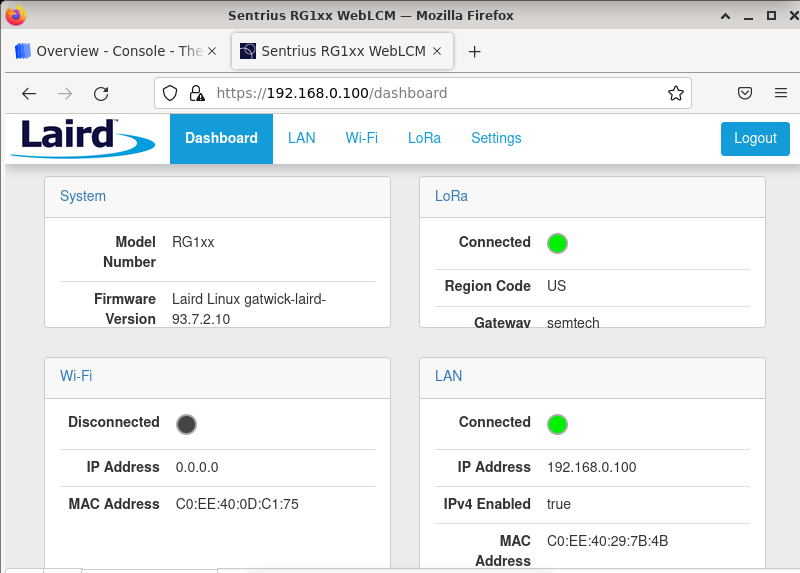
\includegraphics[width=1.0\textwidth]{imagenes/imagenes_manual/mainpagerg191.png}
    \caption{Página principal del RG191}
    \label{fig:rg191-pagina-principal}
\end{figure}

Haga clic en la pestaña LAN y rellénelo con la siguiente información y guárdelo (Figura \ref{fig:rg191-ip-estatica}).

\begin{figure}[H]
    \centering
    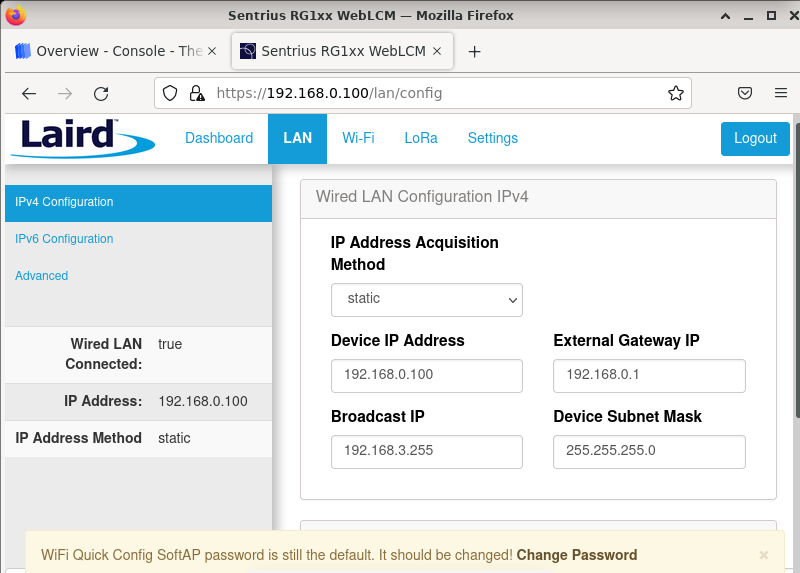
\includegraphics[width=1.0\textwidth]{imagenes/imagenes_manual/modifystatic.png}
    \caption{Modificación de IP Estática en el RG191}
    \label{fig:rg191-ip-estatica}
\end{figure}

Luego haga clic en LoRa y luego en la sección Forwarder y complete con la siguiente información y guárdela (Figura \ref{fig:rg191-lora-forwarder}).

\begin{figure}[H]
    \centering
    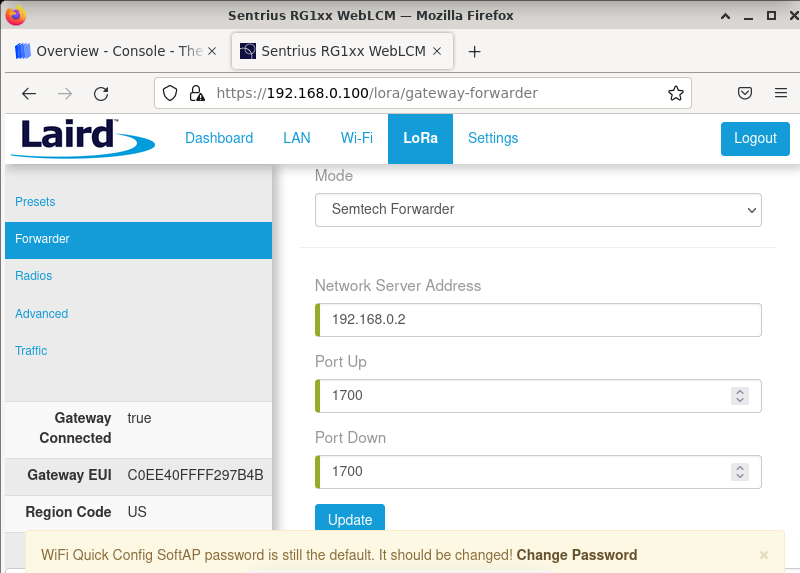
\includegraphics[width=1.0\textwidth]{imagenes/imagenes_manual/modifylora.png}
    \caption{Modificación del protocolo LoRa en el RG191}
    \label{fig:rg191-lora-forwarder}
\end{figure}

Ahora regrese al servidor, debemos verificar las interfaces disponibles para usar para comunicarnos con la puerta de enlace para hacerlo, usamos el siguiente comando

\begin{lstlisting}
    ip link show
\end{lstlisting}

En nuestro caso vamos a usar enp3s0 como interfaz para comunicarnos con la puerta de enlace para modificarla use el siguiente comando

\begin{lstlisting}
    sudo vim /etc/network/interfaces
\end{lstlisting}

Agregue la siguiente información al final del archivo y guárdelo (Figura \ref{fig:interfaz-enp3s0}).

\begin{figure}[H]
    \centering
    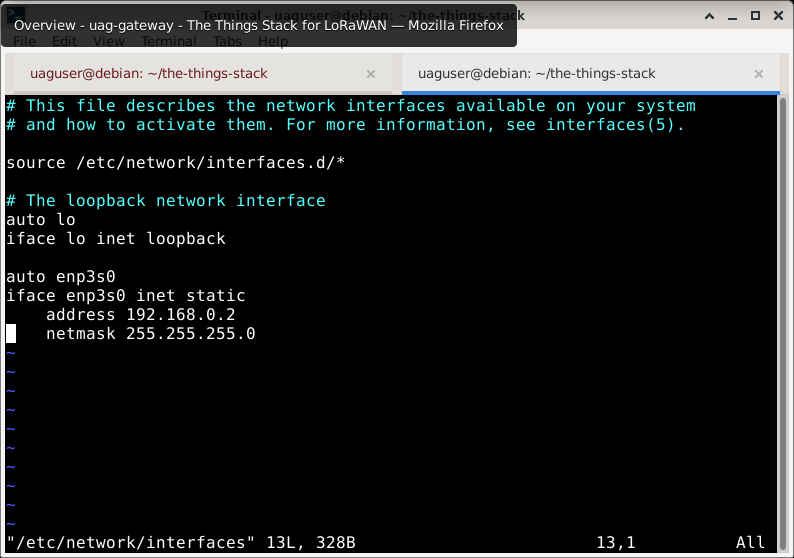
\includegraphics[width=1.0\textwidth]{imagenes/imagenes_manual/staticIP.png}
    \caption{Interfaz enp3s0}
    \label{fig:interfaz-enp3s0}
\end{figure}

Reinicie interfaces de red

\begin{lstlisting}
    sudo systemctl restart networking.service
\end{lstlisting}

Verifique que los cambios se aplicaron en la interfaz de red, en nuestro caso usamos enp3s0

\begin{lstlisting}
    ip -f inet addr show enp3s0
\end{lstlisting}

Verifique la conectividad entre Gateway y Server con el siguiente comando

\begin{lstlisting}
    ping 192.168.0.100
\end{lstlisting}

\textit{Si el ping no es exitoso, verifique nuevamente si la puerta de enlace y la interfaz están configuradas correctamente. Nota: debe perder el acceso a Internet después de este punto si usa IP privadas debido al cambio de IP de la interfaz.}

\subsection{Configurar imágenes de Docker}

Una vez que la puerta de enlace y el servidor de Laird estén configurados con direcciones IP estáticas, ahora estamos listos para configurar nuestras imágenes de Docker

Primero necesitamos migrar la base de datos.

\begin{lstlisting}
    sudo docker-compose run --rm stack is-db migrate
\end{lstlisting}

Ahora cree y administre el usuario para el panel web

\begin{lstlisting}
    sudo docker-compose run --rm stack is-db create-admin-user 
    --id admin --email yourmail@gmail.com
\end{lstlisting}

Luego habilite oauth en el panel web

\begin{lstlisting}
    sudo docker-compose run --rm stack is-db create-oauth-client     --id cli     --name "Command Line Interface"     --owner admin     --no-secret     --redirect-uri "local-callback" 
\end{lstlisting}

Cree estas dos variables de entorno para la contraseña de la consola y para la dirección del servidor

\begin{lstlisting}
    CONSOLE_SECRET="console"
    SERVER_ADDRESS="192.168.0.2"
\end{lstlisting}

Generar usuario autenticado

\begin{lstlisting}
    sudo docker-compose run --rm stack is-db create-oauth-client
    --id console --name "Console" --owner admin --secret 
    "${CONSOLE_SECRET}" --redirect-uri "${SERVER_ADDRESS}/console/
    oauth/callback" --redirect-uri "/console/oauth/callback" 
    --logout-redirect-uri "${SERVER_ADDRESS}/console"  
    --logout-redirect-uri "/console" 
\end{lstlisting}

Ahora estamos listos para ejecutar todos los contenedores.

\begin{lstlisting}
    sudo docker-compose up
\end{lstlisting}

Si todo es exitoso, deberíamos poder acceder al tablero en el siguiente enlace

\begin{lstlisting}
    https://192.168.0.2/console/
\end{lstlisting}

Ahora es el momento de pasar a configurar los dispositivos en el panale web


\section{Configurar panel web}

Una vez que accedemos al tablero desde el navegador, la primera página que deberíamos ver se verá así (Figura \ref{fig:tts-login-page}).

\begin{figure}[H]
    \centering
    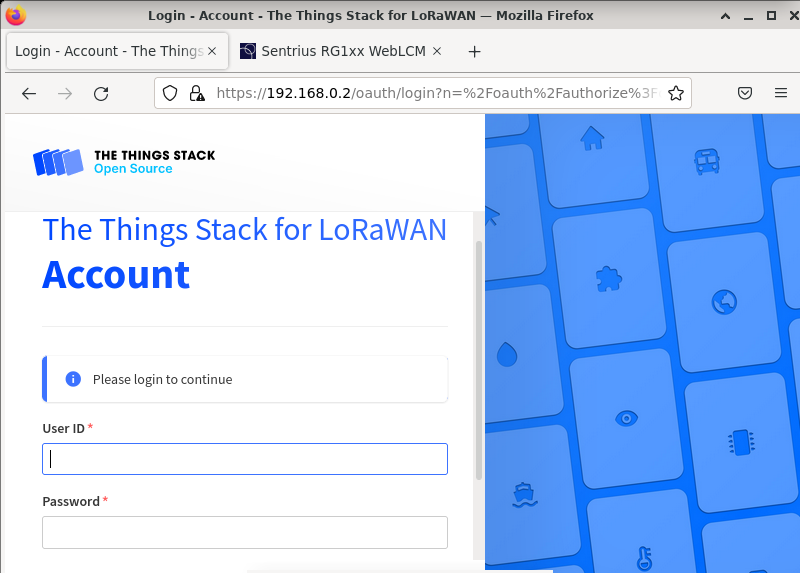
\includegraphics[width=1.0\textwidth]{imagenes/imagenes_manual/loginpage.png}
    \caption{Página principal de The Things Stack}
    \label{fig:tts-login-page}
\end{figure}

Use sus credenciales de administrador que generó previamente para iniciar sesión

\subsection{Registrar puerta de enlace}

Ahora, en la consola principal, haga clic en ir a las puertas de enlace (Figura \ref{fig:gateways-menu}).

\begin{figure}[H]
    \centering
    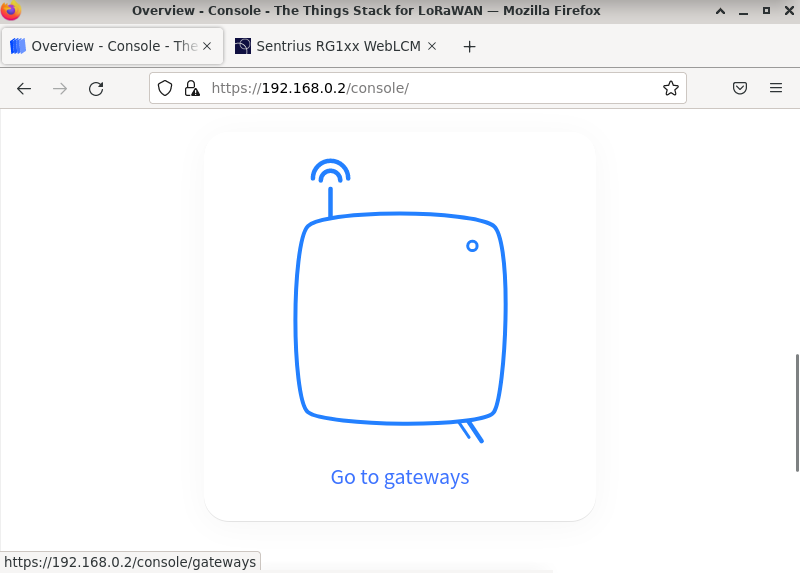
\includegraphics[width=1.0\textwidth]{imagenes/imagenes_manual/gotogateways.png}
    \caption{Icono de la sección \textit{gateways} en el panel web}
    \label{fig:gateways-menu}
\end{figure}

Ahora haga clic en registrar una puerta de enlace (Figura \ref{fig:gateways-list}).

\begin{figure}[H]
    \centering
    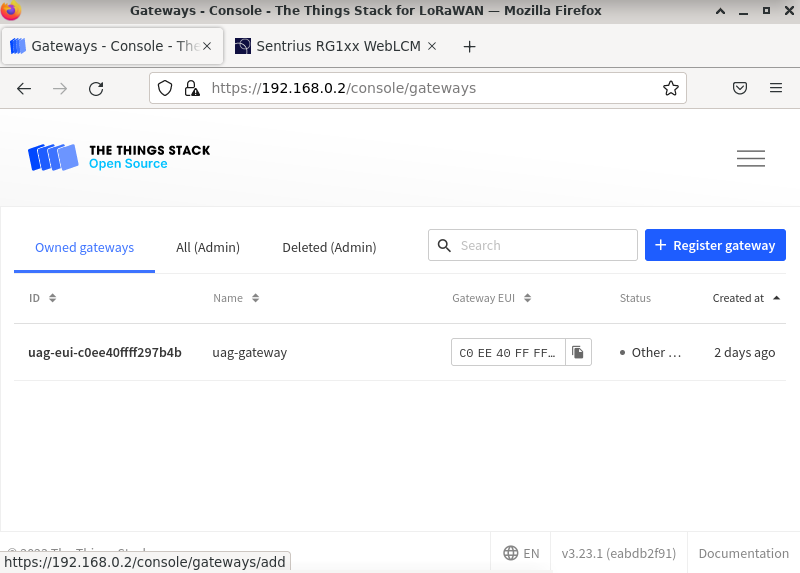
\includegraphics[width=1.0\textwidth]{imagenes/imagenes_manual/clickonregistergateway.png}
    \caption{Sección con el listado de todos los \textit{gateways} en el panel web}
    \label{fig:gateways-list}
\end{figure}

Complete los datos con su EUI correspondiente, ID de puerta de enlace y nombre de puerta de enlace, así como el plan de frecuencia (Figuras \ref{fig:gateway-register-top} y \ref{fig:gateway-register-bottom}).

\begin{figure}[H]
    \centering
    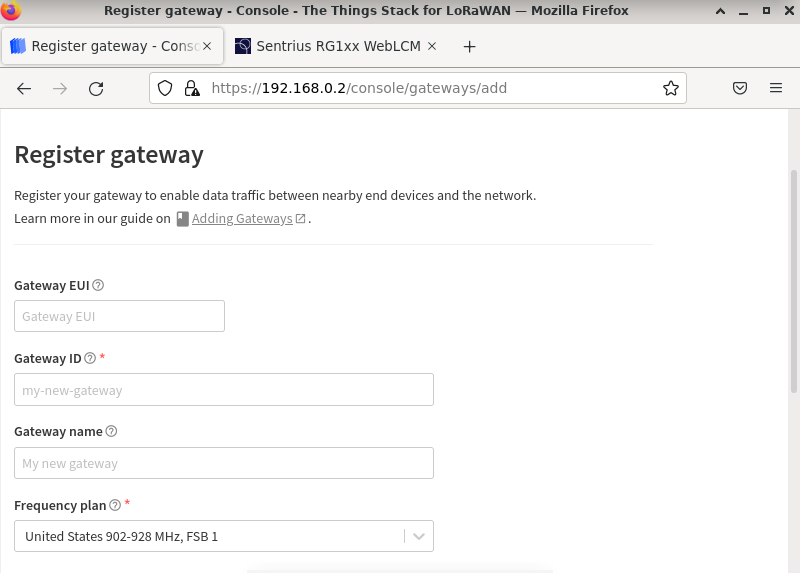
\includegraphics[width=1.0\textwidth]{imagenes/imagenes_manual/registergateway1.png}
    \caption{Sección superior de configuración para registro de un \textit{gateway}}
    \label{fig:gateway-register-top}
\end{figure}

\begin{figure}[H]
    \centering
    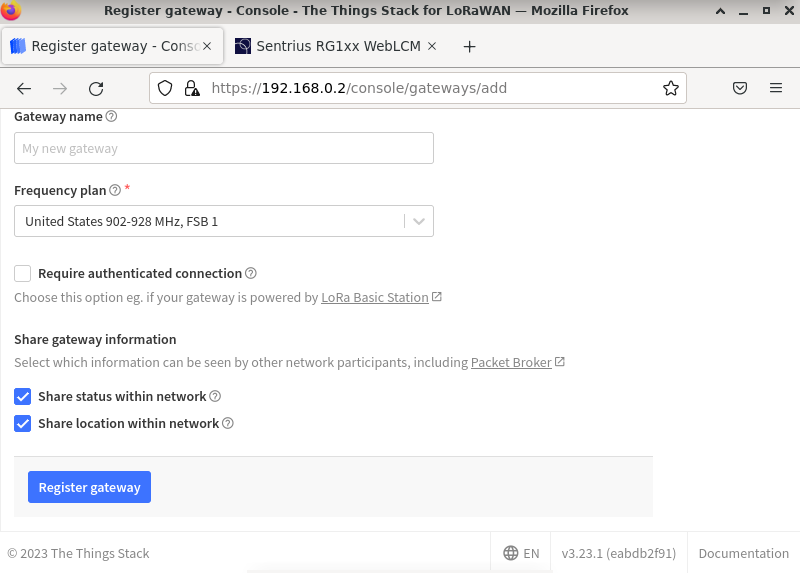
\includegraphics[width=1.0\textwidth]{imagenes/imagenes_manual/registergateway2.png}
    \caption{Sección inferior de configuración para registro de un \textit{gateway}}
    \label{fig:gateway-register-bottom}
\end{figure}

Haga clic en registrar puerta de enlace y ahora debería ver una puerta de enlace como esta (Figura \ref{fig:gateway-configured}).

\begin{figure}[H]
    \centering
    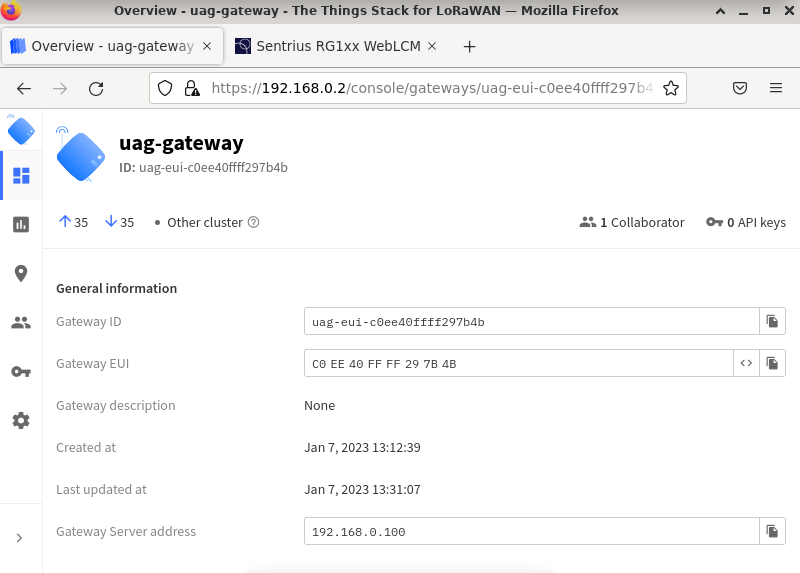
\includegraphics[width=1.0\textwidth]{imagenes/imagenes_manual/finishedgateway.png}
    \caption{Vista de un \textit{gateway} configurado}
    \label{fig:gateway-configured}
\end{figure}

También recuerde deshabilitar la conexión autenticada en caso de que quiera probar nuevos dispositivos LoRa sin credenciales (Figura \ref{fig:gateway-auth-disable}).

\begin{figure}[H]
    \centering
    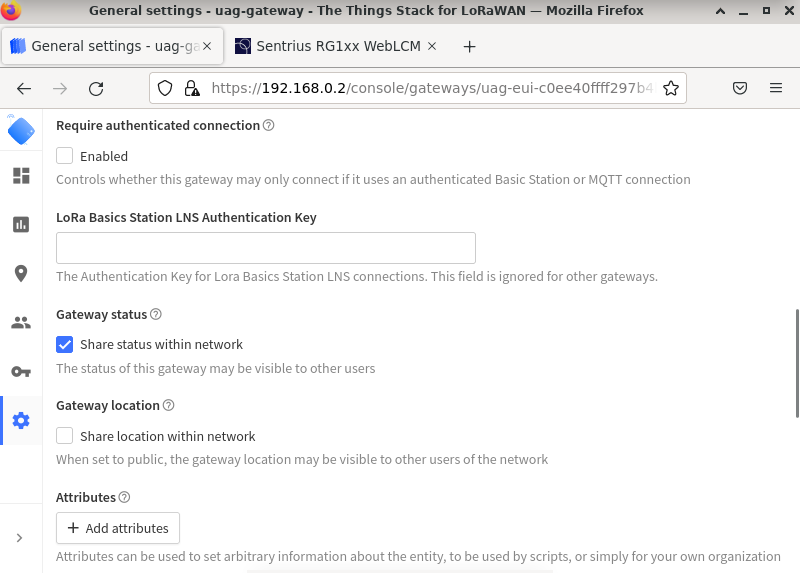
\includegraphics[width=1.0\textwidth]{imagenes/imagenes_manual/disableauth.png}
    \caption{Panel para desactivación de autenticación}
    \label{fig:gateway-auth-disable}
\end{figure}

Ahora puede ver que todo fue exitoso una vez que comenzó a recibir datos en vivo (Figura \ref{fig:gateway-traffic}) de su puerta de enlace (esto puede demorar hasta 1 o 2 minutos dependiendo de la latencia).

\begin{figure}[H]
    \centering
    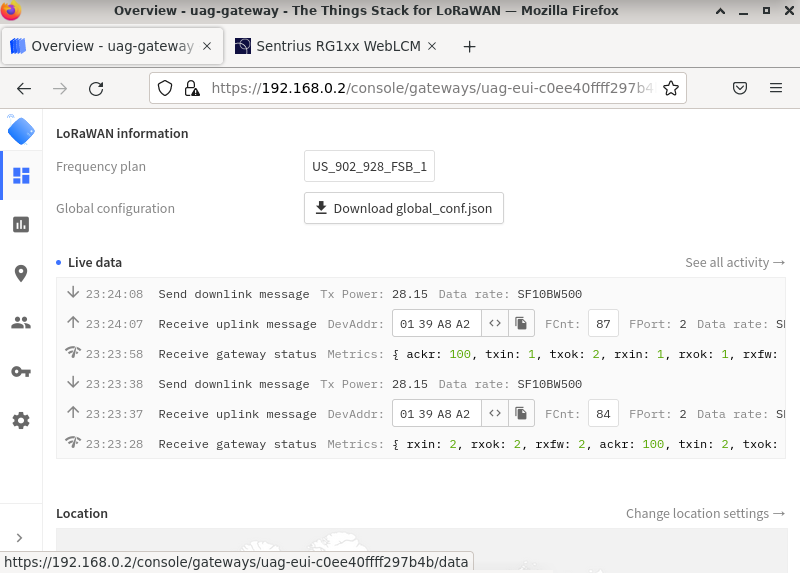
\includegraphics[width=1.0\textwidth]{imagenes/imagenes_manual/trafficgateway.png}
    \caption{Trafico de la red interceptado en el \textit{gateway}}
    \label{fig:gateway-traffic}
\end{figure}

\textit{Recuerda que si aún no tienes dispositivos solo verás mensajes administrativos}

\subsection{Crear una aplicación}

Ahora estamos listos para configurar una aplicación, esto se usa para encapsular todos los dispositivos en un solo punto y tomar información. Para hacerlo, regrese a la página principal de la consola y haga clic en ir a aplicaciones (Figura \ref{fig:applications-menu}).

\begin{figure}[H]
    \centering
    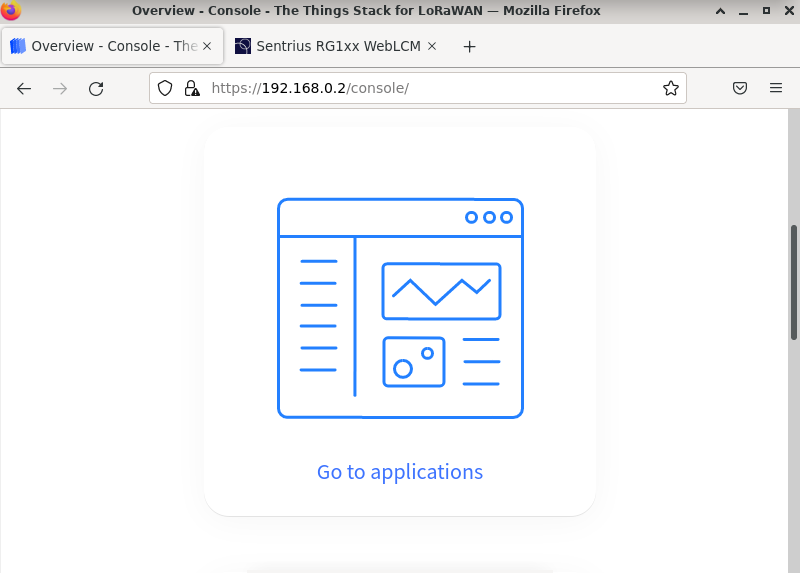
\includegraphics[width=1.0\textwidth]{imagenes/imagenes_manual/gotoapps.png}
    \caption{Icono de la sección \textit{applications} en el panel web}
    \label{fig:applications-menu}
\end{figure}

Haga clic en crear una aplicación (Figura \ref{fig:applications-list}).

\begin{figure}[H]
    \centering
    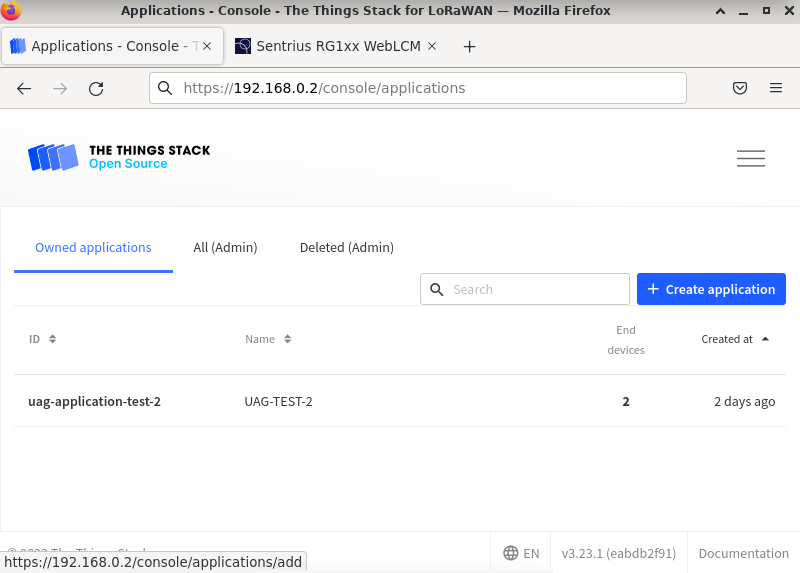
\includegraphics[width=1.0\textwidth]{imagenes/imagenes_manual/createapp.png}
    \caption{Sección con el listado de todos los \textit{applications} en el panel web}
    \label{fig:applications-list}
\end{figure}

Rellénelo con información básica sobre su aplicación y asígnele una identificación única (Figura \ref{fig:application-config}).

\begin{figure}[H]
    \centering
    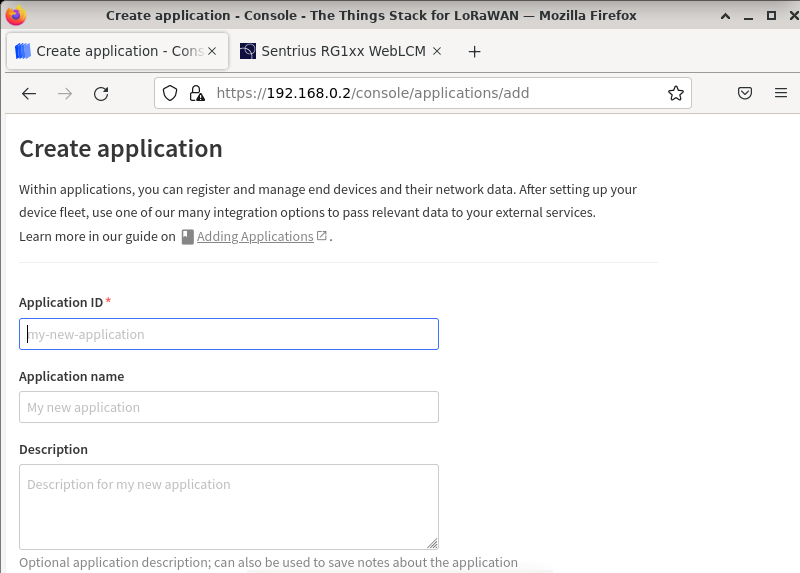
\includegraphics[width=1.0\textwidth]{imagenes/imagenes_manual/createapp2.png}
    \caption{Sección de configuración para registro de un \textit{application}}
    \label{fig:application-config}
\end{figure}

Una vez hecho esto, será redirigido a la página de su aplicación (Figura \ref{fig:application-view}).

\begin{figure}[H]
    \centering
    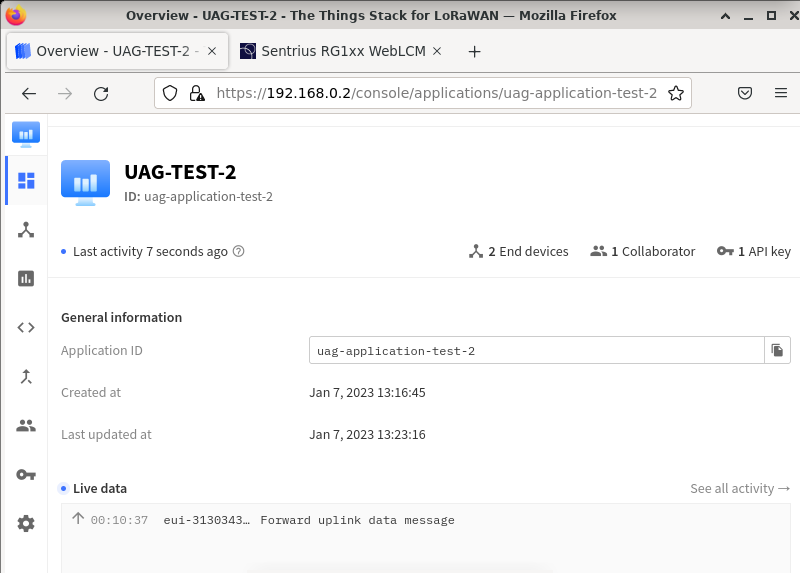
\includegraphics[width=1.0\textwidth]{imagenes/imagenes_manual/apppage.png}
    \caption{Vista de una \textit{application} configurada}
    \label{fig:application-view}
\end{figure}

\subsection{Registrar un nuevo dispositivo}

Ahora necesitamos agregar algunos nodos o dispositivos a nuestra aplicación para comenzar a capturar datos. Haga clic en Dispositivos finales en la columna izquierda de su aplicación y será redirigido a algo como esto (Figura \ref{fig:device-section}).

\begin{figure}[H]
    \centering
    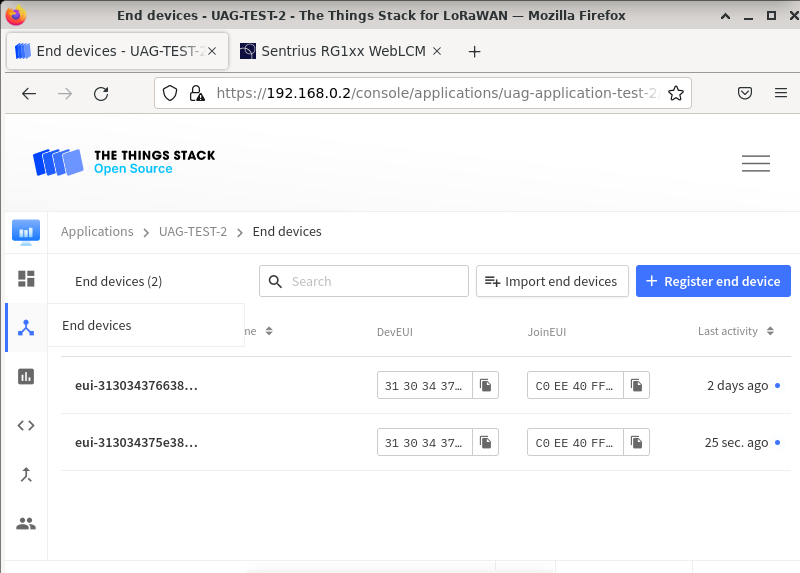
\includegraphics[width=1.0\textwidth]{imagenes/imagenes_manual/enddev.png}
    \caption{Sección superior de configuración para registro de un \textit{device}}
    \label{fig:device-section}
\end{figure}

Haga clic en Registrar dispositivo final y será redirigido nuevamente al formulario de registro de dispositivo final, haga clic en ingresar manualmente los detalles del dispositivo final (Figura \ref{fig:device-register}).

\begin{figure}[H]
    \centering
    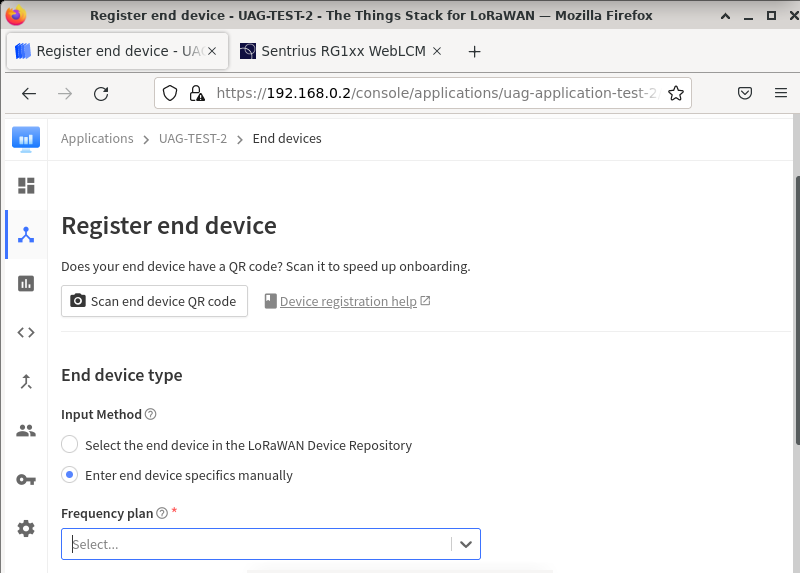
\includegraphics[width=1.0\textwidth]{imagenes/imagenes_manual/registerenddev.png}
    \caption{Sección superior de configuración para registro de un \textit{device}}
    \label{fig:device-register}
\end{figure}

Seleccione el plan de frecuencia adecuado y la especificación LoRaWAN (Figura \ref{fig:device-frequency}).

\begin{figure}[H]
    \centering
    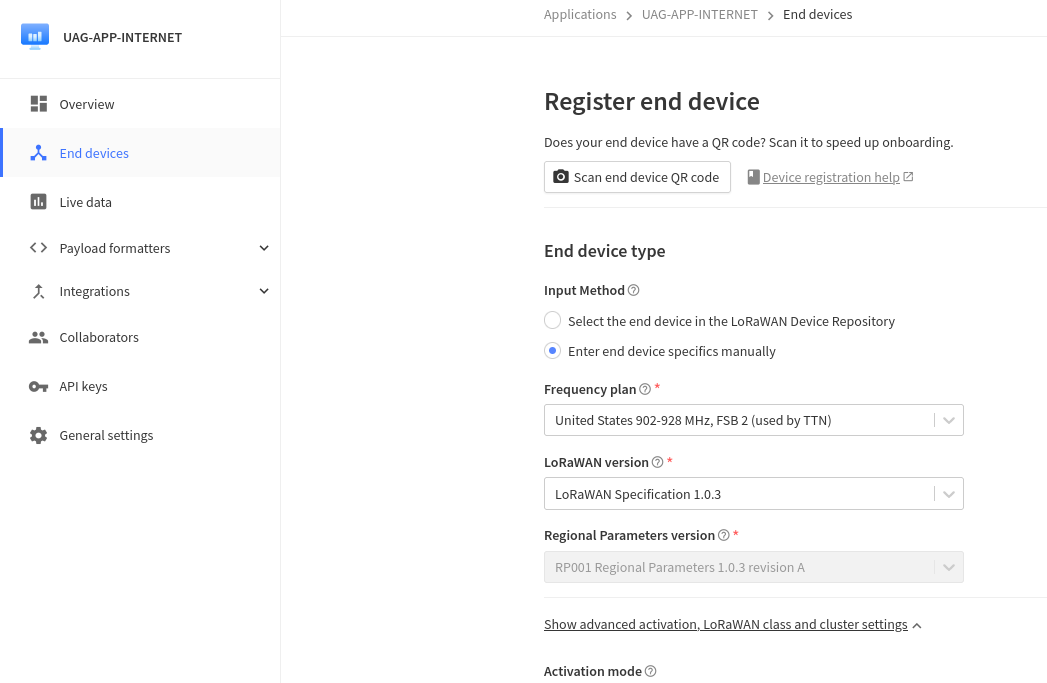
\includegraphics[width=1.0\textwidth]{imagenes/imagenes_manual/registerenddev2.png}
    \caption{Sección de frecuencia de configuración para registro de un \textit{device}}
    \label{fig:device-frequency}
\end{figure}

Debido a errores en la implementación, recomendamos el uso de 1.0.3.

Use activación de aire OTAA y clase A únicamente, también mantenga la configuración predeterminada de MAC (Figura \ref{fig:device-otaa}).

\begin{figure}[H]
    \centering
    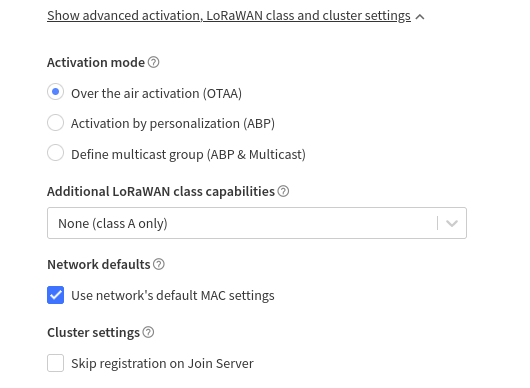
\includegraphics[width=1.0\textwidth]{imagenes/imagenes_manual/registerenddev3.png}
    \caption{Sección media de configuración para registro de un \textit{device}}
    \label{fig:device-otaa}
\end{figure}

Agregue JoinEUI, este es básicamente el mismo EUI que viene con su puerta de enlace que se usa para comunicarse en ambos sentidos (Figura \ref{fig:device-join-eui}).

\begin{figure}[H]
    \centering
    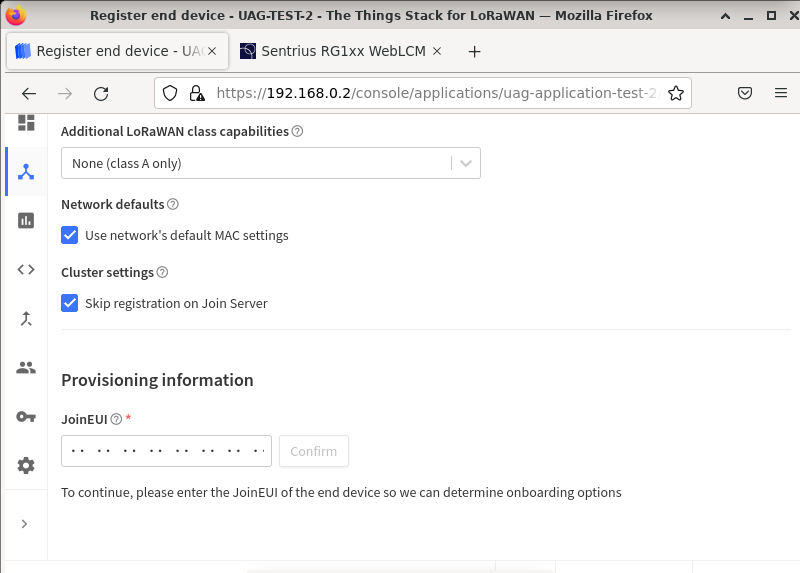
\includegraphics[width=1.0\textwidth]{imagenes/imagenes_manual/registerenddev4.png}
    \caption{Sección inferior de configuración para registro de un \textit{device}}
    \label{fig:device-join-eui}
\end{figure}

Haga clic en confirmar y ahora podrá ver el dispositivo en su aplicación, así como acceder a él (Figura \ref{fig:device-configured}).

\begin{figure}[H]
    \centering
    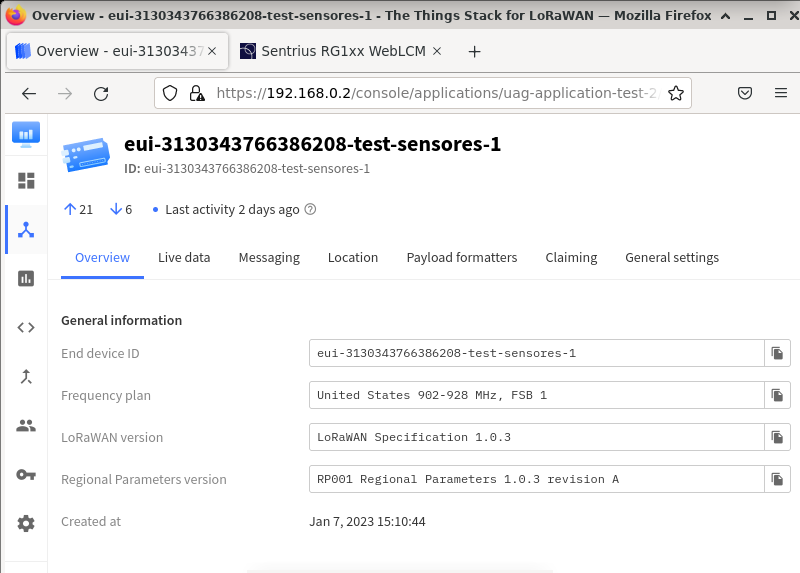
\includegraphics[width=1.0\textwidth]{imagenes/imagenes_manual/deviceexample.png}
    \caption{Vista de un \textit{device} configurado}
    \label{fig:device-configured}
\end{figure}

Ahora todo está configurado, Conecte su dispositivo a la corriente y comenzará a recibir datos en poco tiempo justo como en la siguiente imagen (Figura \ref{fig:device-live-data}).

\begin{figure}[H]
    \centering
    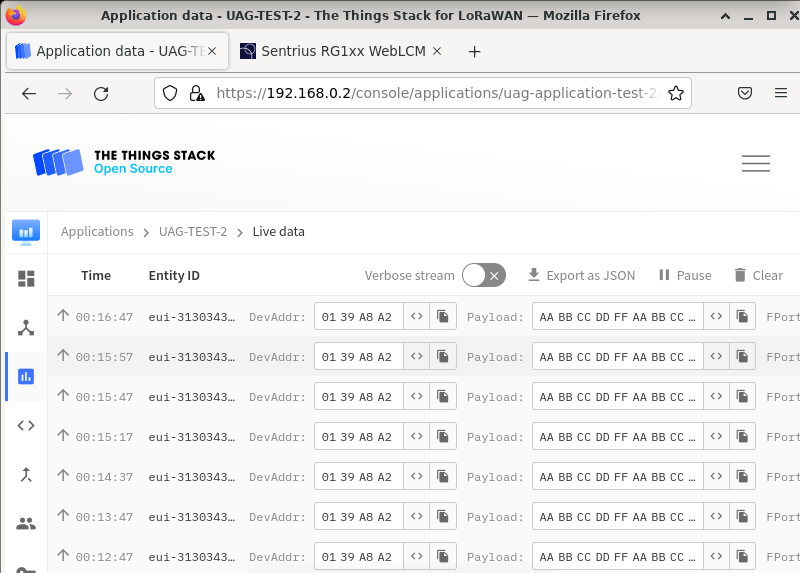
\includegraphics[width=1.0\textwidth]{imagenes/imagenes_manual/livedatafromnode.png}
    \caption{Vista de un \textit{device} configurado}
    \label{fig:device-live-data}
\end{figure}

\subsection{Leer información usando Linux}

Una vez lanzadas todas las herramientas explicadas en los capítulos anteriores podemos notar que empezamos a recibir información a través del panel web (Figura \ref{fig:device-live-data}) sin embargo podemos extender su funcionalidad leyendo la información utilizando la terminal de comandos. Gracias a esto, podemos tomar generar capas extra de funcionalidad.

La lectura de información del panel web se hace a través de su interfaz de programación de aplicaciones, utilizando el comando curl:

\begin{lstlisting}
    curl --cacert cert.pem \
    "https://192.168.0.2/api/v3/events" \
    -X POST -H "Authorization: Bearer $API_KEY" \
    -H "Accept: text/event-stream" \
    -H 'Connection: keep-alive' \
    --data-raw $'{"identifiers":[{"application_ids":
    {"application_id":"uag-application-test-2"}}]}\n'
\end{lstlisting}

El comando se compone de múltiples opciones.

La primer linea llama el comando curl asi como su certificado \textit{cert.pem} (Generado previamente para el lanzamiento del panel web)

La segunda linea utiliza la dirección IP del panel web con la ruta \textit{/api/v3/events}

La tercera linea habla del método de llamada \textit{POST} asi como del uso de la variable \textit{API\_KEY} la cual es generada a través del panel web.

La cuarta linea describe el método de comunicación el cual usara un flujo de datos por eventos basados en texto

La quinta linea especifica el mantener la conexión viva y funcionando mientras sigamos necesitando datos.

Por ultimo las dos últimas líneas describen los datos que obtendremos de la interfaz, los cuales son datos de la aplicación \textit{uag-application-test-2}, estos pueden ser modificados consultando la documentación oficial de la interfaz. 

Una vez obteniendo los datos obtendremos una cadena de texto tipo JSON, en la cual podremos encontrar múltiples datos relacionados a la llamada entre servidor y nodo, para nuestros propósitos el mas importante es el llamado payload. Este son los datos encriptados del nodo, los cuales están codificados en base64 para su mayor seguridad. Podemos desencriptarlos con alguna herramienta web o utilizando el programa en Python que se vera en la siguiente sección.

\subsection{Leer información usando código en Python}

Una capa extra añadida en nuestra investigación es el uso de un programa automatizado para la recopilación y administración de datos, como prerrequisito necesitamos apoyarnos del comando de Linux que vimos en la sección anterior y enviar los datos a un archivo con el uso del redireccionamiento de datos o con el operador doble mayor que. \[ \gg \]

Una vez que dejemos corriendo este comando empezaremos a recabar datos en un archivo de manera continua y estaremos listos para correr nuestro programa en Python. El cual nos ayuda a separar la información y agregar personalización dependiendo de los requisitos de los usuarios.

El código es el siguiente:


\begin{lstlisting}
#!/usr/bin/env python 

"""
This script is used to retrieve last data from server API and send it
to a desired dashboard.

Usage: python middleware.py
"""
import requests
import json
import base64

#INDEXES MEANING
DEVICE_ID   = 0
PAYLOAD     = 1
# URL Where are you storing logs of the server
# Feel free to change to suit your needs
SERVER_LOGS_PATH='/tmp/logs_pako.txt'

# External dashboard URL and headers
# Feel free to modify it to suit your needs
dashboard_url = "https://sistema-incendios-uag.up.railway.app\
/api/nodes-data"
dashboard_headers = {
    'Accept'        : 'application/json',
    #API_KEY
    'Authorization' : 'Bearer 7|yvXruJRQtoWNqsNZYQQdrmLqNj69mIg4ej06RkFn', 
    'Content-Type'  : 'application/json'
}

def decrypt_data(string):
    """
    Function to decrypt any data in base64 to binary
    """
    decode_payload = base64.b64decode(string.encode('ascii'))
    return decode_payload.hex()

def call_node_data():
    """
    Read the logs from the watcher
    """
    with open(SERVER_LOGS_PATH, 'r') as f:
        last_line = f.readlines()[-3]
    response = json.loads(last_line)
    #Get the payload
    return [response['result']['identifiers'][0]['device_ids']['device_id'],response['result']['data']['uplink_message']['frm_payload']]

def format_payload(payload, device_id):
    """
    Here we can format the payload to our needs
    """
    #IMPORTANT for this example we are sending all the PAYLOAD as
    #TEMPERATURE it dependes on programmer to split data as needed
    dashboard_payload={
        "node_id": device_id,
        "temperature" : payload,
        # "gas": 69,
        # "humidity": 666,
        # "fire": 420 
    }
    return dashboard_payload

def submit_node_data(data):
    """
    Submit node data to dashboard
    """
    response = requests.post(dashboard_url, 
    json=data, headers=dashboard_headers)
    if response.status_code != 200 | response.status_code != 201:
        print('ERROR: {}. Status code: {}'.format(
        response.reason, response.status_code))
        print('ERROR: {}'.format(response.text))
    return response

if __name__ == '__main__':
    #TODO: add persistant running with while and keep 
    #last line if changed run cycle again, if not skip until 
    #next minute or whatever time we want
    
    # Get data from nodes
    response = call_node_data()
    # Decrypt payload
    raw_payload = decrypt_data(response[PAYLOAD])
    # Format payload
    dashboard_payload = format_payload(raw_payload, 
    response[DEVICE_ID])
    # Print message to be sent
    print(dashboard_payload)
    # Send the message to dashboard
    submit_node_data(dashboard_payload)
\end{lstlisting}

El programa se compone de cuatro funciones principales.

La primera función \textit{call\_node\_data} hace el llamado del archivo donde guardamos los datos, leyendo las ultimas líneas y transformándolas en un objeto JSON para extraer los datos del nodo.

La segunda función \textit{decrypt\_data} nos ayuda a desencriptar los datos en base64 de forma automática, obteniendo una trama legible en texto plano.

Mas adelante la tercera función \textit{dashboard\_payload} nos ayuda a formar una nueva trama la cual será enviada por la función \textit{submit\_node\_data}


\subsection{Problemas comunes encontrados y sus soluciones}

P: ¿Qué debo hacer para instalar Debian sin internet en el servidor?

R: Como el servidor está aislado sin una interfaz Wi-Fi, recomendamos descargar una imagen de \href{https://www.debian.org/CD/http-ftp/}{CD/DVD}, que tiene más memoria, pero la ventaja es que viene con muchas herramientas preconstruidas instaladas como un entorno de escritorio.

P: No puedo conectarme a la URL de API, ¿qué puedo hacer?

R: A partir del 11 de enero de 2023, existe un problema conocido con respecto al archivo ttn, agregue este código a continuación en console.ui Verifique el archivo del repositorio como referencia

\begin{lstlisting}
    dcs:
      base-url: "https://192.168.0.2/api/v3"
\end{lstlisting}

P: Al instalar Go hay un error con una variable llamada GOPATH que no me deja continuar, ¿qué puedo hacer?

R: Si se configura GOPATH, se producirá un error al eliminar esta variable.

\begin{lstlisting}
    unset GOPATH
\end{lstlisting}

P: Al instalar Go, hay un error con respecto al comando make.

R: En caso de que no tenga el comando make, instale las herramientas esenciales en Debian, el comando es

\begin{lstlisting}
    sudo apt-get install build-essential
\end{lstlisting}

P: No puedo iniciar el tablero usando Redactar debido a un puerto de error

R: A veces, otros servicios toman algunos puertos necesarios para que el tablero funcione para verificar qué servicios están actualmente tomando puertos y ejecutándose, use el siguiente comando

\begin{lstlisting}
    sudo ss -nlpt
\end{lstlisting}

En nuestro caso, apache2 estaba tomando el puerto 80, por lo que necesitamos detenerlo.

\begin{lstlisting}
    sudo service apache2 stop
\end{lstlisting}

P: Completé la información de la puerta de enlace pero no se registró

R: A veces, la información de la puerta de enlace no se registra como se esperaba y tenemos que modificarla manualmente. Para hacerlo, vaya a la configuración y modifique el campo de dirección del servidor de la puerta de enlace (Figura \ref{fig:gateway-ip-settings}).

\begin{figure}[H]
    \centering
    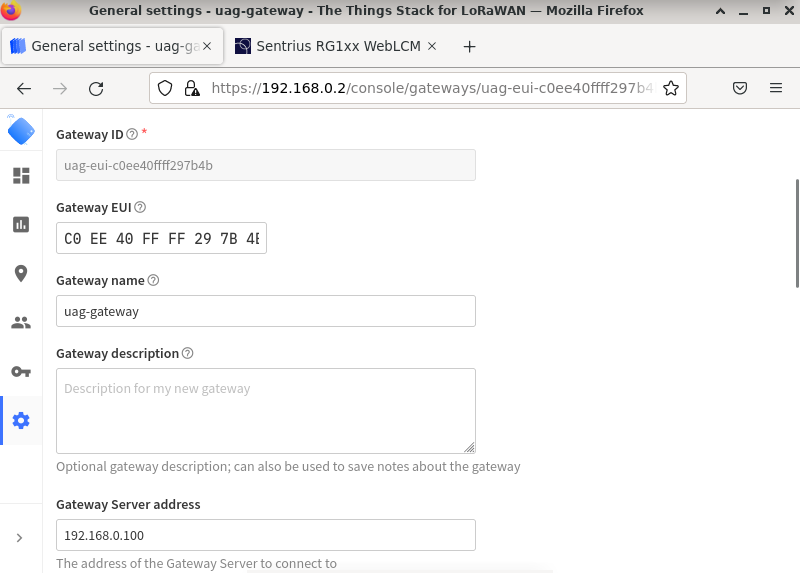
\includegraphics[width=1.0\textwidth]{imagenes/imagenes_manual/changestaticIP.png}
    \caption{Vista de configuración para la IP de un \textit{gateway}}
    \label{fig:gateway-ip-settings}
\end{figure}

P: No puedo entender que la carga útil parece estar encriptada

R: Puede deshabilitar los formateadores de la carga útil para ver los datos sin formato en caso de que quiera probar. Vaya a formateadores de carga útil en su dispositivo y seleccione Ninguno (Figura \ref{fig:payload-format-view}).

\begin{figure}[H]
    \centering
    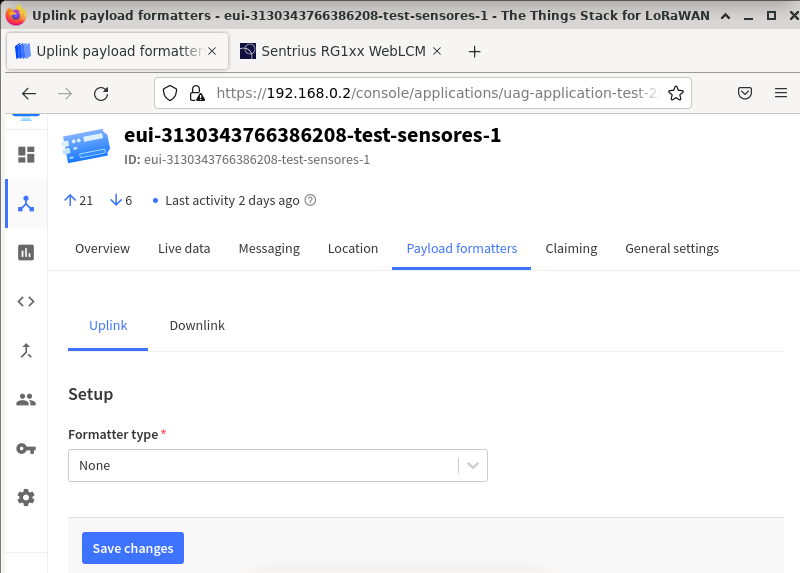
\includegraphics[width=1.0\textwidth]{imagenes/imagenes_manual/disablepayloadformatters.png}
    \caption{Vista para el formato de los paquetes}
    \label{fig:payload-format-view}
\end{figure}

Guardar los cambios

P: La aplicación no me permite registrar un dispositivo porque ya está en uso

R: Cambie el EUI de su dispositivo y cambie la ID del dispositivo una vez que se registre en la aplicación

P: No puedo revisar los mensajes de datos en vivo en el tablero

R: A veces, este problema se debe a que la puerta de enlace no puede comunicarse con los nodos, verifique dos veces los EUI de la puerta de enlace y los dispositivos e intente volver a conectarse con la puerta de enlace usando el comando ping a la IP.    % Capitulo 03

        \chapter{Conclusiones}
        %Capítulo 4

\section{Conclusiones y las recomendaciones}

En este ultimo capitulo se habla sobre las conclusiones obtenidas durante la investigación, su
desarrollo, logros conseguidos y proyectos futuros que puedan surgir de este.

    \textbf{\textit{Descripción}}

En este proyecto se ha diseñado todo un flujo de trabajo que hace uso de la tecnología LoRaWAN, se
ha buscado la generalización par que distintos usuarios, investigadores o empresas puedan usarlo en
sus monitoreos y obtener distintas métricas asi como tomar acciones en base a estos datos. Además de
ello, los programas desarrollados propuestos pueden ser escalables a distintos tipos de
funcionalidades e inclusive tecnologías.

Como primer punto, se hizo una investigación de la tecnología LoRa y LoRaWAN y se resalto el como
esta puede funcionar en equipos mínimos a grandes distancias utilizando pocos recursos. Se procedió
al desarrollo conjunto de una solución embebida al mismo tiempo que se montaba y configuraba un
servidor maestro que puede ser escalable a múltiples servidores con múltiples nodos. Una vez
teniendo todo configurado todo el sistema se pasó a la programación de una capa superior para la
especialización de estos nodos por dos equipos de investigadores distintos demostrando asi su
capacidad de adaptación para futuros proyectos con el minimo esfuerzo.

Teniendo todo el trabajo se pasó al paso de pruebas de todo el flujo de trabajo obteniendo datos
desde múltiples nodos siendo procesados y enviados a los paneles web para finalmente ser desplegados
apropiadamente, demostrando de esta forma la robustez del sistema. Además de la documentación de
todos estos procedimientos no solo en este trabajo si no en un repositorio privado para los
investigadores involucrados en el proyecto.

    \textbf{\textit{Trabajos futuros}}

A pesar de la robustes del flujo de trabajo, hay cabida para múltiples puntos de mejora o distintas
soluciones extras y capas de funcionalidad que pueden ser implementadas en base a distintos
requisitos.
\begin{itemize}
    \item Montaje de un servidor de servidores en la nube.
    \item Orquestación de contenedores asi como balanceo de cargas entre ellos.
    \item Análisis del rendimiento y coste energético del sistema para la búsqueda de optimización en estas áreas. 
    \item Implementar una solución más compacta para continuar simplificando su funcionalidad en usuarios finales.
\end{itemize}
    % Capitulo 04

        %\chapter{Referencias}
        %\section{Referencias documentales}

\textbf{\textit{Descripción}}

Es el listado de libros, documentos, reportes de investigación, gráficos, tablas, etc.

\textbf{\textit{Criterios de calidad}}

Debe citar técnicamente la bibliografía base de la investigación.

%\section{Código fuente {\it miprograma.c}}
El siguiente código se importó directamente del archivo % {\it miprograma.c}

%\inputminted[breaklines=true]{c}{codigo/miprograma.c} 

        \bibliographystyle{ieeetr} % Formato de la IEEE
        \phantomsection
        \addcontentsline{toc}{chapter}{\bibname}
        \bibliography{bibliografia/articulos,bibliografia/libros,bibliografia/miscellaneous}

    \end{document}
%-----------------------------------------------------------%
